\documentclass[
  utf8,%     More capable input encoding than latin-1.
  % parskip,%  For vertical whitespace between paragraphs.  This comes down to more than just using parskip.sty, so it's better to use this class option.
  % S5MP % If you intend to really use margin paragraphs (not recommended!).
%  crop,%     Produce output with crop marks and paper size A4.  Liu-Tryck should like this.  Automatically adds information, including the physical page number, at the top of each page.
       %     Add option 'noInfo' to suppress the info at the top of each page when using option 'crop'.
  % Font options: 'kp' (default), 'times', 'lm'.  The KpFonts (loaded using 'kp'), is the most complete font among the provided options.  Among other, it supports slanted small caps.  See rtthesis.cls for more details regarding the font options.
  largesmallcaps,widermath,% Good options to KpFonts.
  sharecounter,nobreak,definition=marks,%  See comments in the results chapter of this document for more information on these options!
  %numbers, % If you want to cite references by numbers, use this option.
  noparts% Use option 'noparts' if you do not make use of part divisions.
]{rtthesis}

\usepackage{mythesis}

\begin{document}

\selectlanguage{english}
\makeFrontPage
\frontmatter
\maketitlegit
\makeLibraryPage{The number of connected devices connected to the Internet is growing rapidly, when talking about devices it also contains the once not having any contact with humans. This types of devices is the once that is expected growing the most. That is why the field of device fingerprinting is an area that which require more investigation. This thesis measure and evaluates the use of the accelerometer, camera and gyroscope sensors of a mobile device as fingerprinting of a device. The method used is based on previous research in sensor identification together with methods used for designing a biometric system. The combination with long-proven methods in the biometric area with new research of sensor identification is a new approach of looking at device fingerprinting.
}

\begin{abstract}[swedish]
  Antalet anslutna enheter som är anslutna till internet växer snabbt, när man talar om enheter så menar man också de som inte har någon kontakt med människor, ex. en uppkopplad temperaturgivare till en termostat. Denna typer av enheter är de som förväntas växa mest. Vilket är anledningen till att området för att unikt identifiera dessa enheter kräver mer undersökning. Det här exjobbet inkluderar mätningar och utvärdering på användningen av accelerometern, kamera och gyroskop sensorer på en mobil för att undersöka i vilken utsträcning de går att identifiera som unika enheter. Alltså som ett fingeravtryck för sensorer. Den metod som används bygger på tidigare forskning inom sensor identifiering tillsammans med metoder som används för att utforma ett biometriskt system. Kombinationen med långa beprövade metoder inom biometriområdet med ny forskning inom identifiering av sensorer är en nytt sätt för att titta på enheters fingeravtryck.

\end{abstract}
\begin{abstract}[english]
  The number of connected devices connected to the Internet is growing rapidly, when talking about devices it also contains the once not having any contact with humans. This types of devices is the once that is expected growing the most. That is why the field of device fingerprinting is an area that which require more investigation. This thesis measure and evaluates the use of the accelerometer, camera and gyroscope sensors of a mobile device as fingerprinting of a device. The method used is based on previous research in sensor identification together with methods used for designing a biometric system. The combination with long-proven methods in the biometric area with new research of sensor identification is a new approach of looking at device fingerprinting.

\end{abstract}
\begin{acknowledgments}
  I thanks\dots

  \addvspace{1em}
  \begin{flushright}
    \textit{%
      Linköping, June 2015\\
      Anna Karlsson%
    }
  \end{flushright}
\end{acknowledgments}

\tableofcontents
\begin{notation}% Passing the option "old" to the notation environment will redefine the notationtabular environment so that it produces an old style LaTeX tabular instead of a ctable.sty style tabular.
  \centering

  \begin{notationtabular}{Notation}{Notation}{Meaning}
    G\index{G!abbreviation} & G-force \\
    $\epsilon$ & Bias\\
    $\boldsymbol{ F}_C$ & Coriolis force \\
    $T$ & Tesla (SI-unit of magnetic flux density) \\
  \end{notationtabular}

  \begin{notationtabular}{Abbreviations}{Abbreviation}{Meaning}
    FAR\index{FAR!abbreviation} & False Accept Rate \\
    FRR\index{FRR@!abbreviation} & False Reject Rate \\
    FTE\index{FTE!abbreviation} & Fail To Enrollment \\
    ICT\index{ICT@!abbreviation} & Information and Communication Technologies \\
    IoT\index{IoT@!abbreviation} & Internet of Things \\
    M2M\index{M2M!abbreviation} & Machine-to-machine \\
    MEMS\index{MEMS!abbreviation} & Micro-electromechanical System \\
    NIC\index{NIC!abberviation} & Network Interface Card \\
    OS\index{OS!abberviation} & Operating System \\
    PRNU\index{PRNU!abberviation} & Photo-Response Non-Uniformity noise \\
    RMS\index{RMS!abberviation} & Root Mean Square \\
    SVM\index{SVM!abberviation} & Support Vector Machine \\
  \end{notationtabular}
\end{notation}


\mainmatter
\chapter{INTRODUCTION}\label{cha:intro}
This paper is the report for my master thesis in Computer Science and the last part of my education for become an engineer in information-technology in field of secure systems. The thesis was performed on Cybercom AB in Linköping. \\
This introduction chapter will give an overview of the work together with background and aims and objectives that is used as the basis for the work presented in this thesis. 

\section{Background}\label{sec:bg}
Cars, locks, birds, stoves, refrigerator, coffee maker, watches, cat feeder, sewing machines\dots, the world of connected devices is growing rapidly. For making this things connect to each other we need secure authentication methods for knowing that they are connecting to the device they are suppose to and not anything or anyone else. \\
\\
For us humans it has become an everyday thing to using two factor authentication when accessing buildings, part of networks, our bank and so on. When talking about two factor authentication we usually use a combination of either three things; something you \textit{know} like passwords, something you \textit{have} like tag, passport, card or phone, something you \textit{are} like iris or fingerprint. Mot about the in chapter ~\ref{cha:auth}.\\
Something you know or have is things that can be copied, stolen or modified fairly easy and without meet or know all that much about the person or thing you try to authenticate as. This compared to something you are as iris, fingerprint and DNA requires much more effort and time since you can only focus on one person at a time. 

\section{Aims \& Objectives}\label{sec:aim}
Today most of the solutions for M2M authentication involves a certificate, token, UUID etc., from my opinion is this something the machine know or have. The area of fingerprinting a machine has been more investigated in line with the world of IoT (Internet of Things) has grown. The aim of this thesis is to look in to if the fingerprinting methods found today, can be used as something the machine \textit{are} for two factor authentication between them. The problems I'll work to solve with this thesis is:
\begin{itemize}
	\item[] Can you create a device fingerprint by using the unique hardware characteristics in a mobile device?
	\item[] Is this fingerprint suitable for using as a second factor for authentication between devices?
\end{itemize}
The problems above state a mobile device and not a general machine, which is one of my limitations in the area. When stating a mobile device leaves also leads to wireless network environment. The focus is also set to an authentication process where you are able to collect a set of data from the device in a database in a test environment. This means that new devices in the network has to go trough some kind of phase were collecting the unique hardware characteristics data. As the title of the thesis implies, authentication is the focus not identification. Since I'll accomplish some kind fingerprint for the mobile device software, certificates, tokens and types of ID will not be looked in to. This because I think that it's not something the device are, more something it has or knows. \\
\\
There are different point of views to this work and can be summed up to the objectives:
\begin{itemize}
	\item[] \textbf{Explore different unique hardware characteristics of a mobile device} \\
	Mobile devices today are equipped with a lot of sensors and since they like other hardware has some noise that may be unique enough to differ from a device of the same model. Measurements from the microphone-, speaker-, gyroscope-, accelerometer- and camera-sensor will be collected and valuated from the view as fingerprints. RFF (Radio Frequency Fingerprinting) is another perspective that also will be measured from the noise of the mobile devices in a wireless environment and compared together with the sensors.
	\item[] \textbf{Combining M2M, two factor and biometric authentication} \\
	Biometric authentication has ways of measure and compare fingerprints, this measurements and methods will be used to make the two factor authentication between the devices.
\end{itemize}

\section{Thesis Outline}\label{sec:outline}
This introduction chapter including background, aims and objectives will give a quick view of what the thesis is about. The chapters that following is divided in different parts that maps to the different objectives listed above.
\begin{itemize}
	\item[Ch.1: ]	This will give an introduction to the work done in the thesis and motivation for doing it.
	\item[Ch.2: ]	How authentication is made today between machines, two factor and in biometric.
	\item[Ch.3: ]	The different unique hardware characteristics of a mobile device that has been found today and how they are collected.
	\item[Ch.4: ]	Result of the collected unique hardware characteristics of a mobile device together with comparison and evaluation on if they can be used as mobile fingerprints or not. This chapter also presents the demo the made from the test result.
	\item[Ch.5: ]	Conclusion will except conclusions also include ethical aspects and further work. 
\end{itemize}


\section{Related Work}\label{sec:relatedWork}
TODO! or to be removed and covered in the next two chapters...
\chapter{COMMUNICATION \& AUTHENTICATION}\label{cha:auth} \index{authentication}
Because just about all devices that are connected to a network are one way or another connected to the Internet you can bet that they find themselves in an untenanted or malicious environment. Everything connected to the Internet is very likely to be hacked. Thus, authentication is needed for remote sensing devices to communicate. \cite[]{auth:M2Mcom}\\
In this chapter will show ways of authentication (two factor, M2M and biometric) that is in the area of this thesis. The biometric part is in the area because it has good ways of measure strength in a biometric trait (especially fingerprint) that will be used when comparing strength of my tests of characteristic noise in the mobile device.

\section{Two factor authentication}\label{sec:2fauth} \index{two factor authentication}
There are more ways to authenticate a user than password, however it is the most common. There are three different types of authentication; 
\begin{itemize}
	\item Something the authenticator \textit{have} like a key, card, passport and so on
	\item Something the authenticator \textit{knows} for example password
	\item Something the authenticator \textit{are}, known as biometrics such as fingerprint or iris pattern
\end{itemize}
\cite[p.~31]{rosssec} \\
Authentication in two factor means a combination of two of the three types of authentication above. An example can be use of a credit card (you have) in combination with a PIN-code (you know) to collect the money from an ATM. Something the authenticator have and knows is the most common combination. The third one, cost is the biggest reason form that biometrics isn't that common yet.
\cite[p.~47]{rosssec}

\section{Challenge-Response authentication}\label{sec:challResp} \index{challenge-response}
The challenge-response protocol is build upon the idea that the user to a system first must complete a challenge decided by the system in order to access the system. An example is modern car keys when trying to start the engine, the engine controller give the key an challenge consisting of a random $n$-bit number. The key encrypt the challenge and response. \\
The problem challenge-response protocols facing is often to achieve good randomness, thus is the challenge not random enough there is a risk for malicious user to calculate the $n$-bit number. \\
There are other applications than looks, like the HTTP Digest Authentication. It uses the authentication process  which a web server challenges a client or a proxy with the common secret of a password. The server sends nonce to the client or proxy, whom hash the nonce with the password and the requested URI. This authentication mechanism is not vulnerable to password snooping and is used in cases like; client-server-authentication in SIP or the protocol for Voice-Over-IP telephony. This protocol however is vulnerable to man-in-the-middle. \\
\\
Ross states however that a much more visible use of challenge response is in \textit{two-factor authentication} (~\sectionref{sec:2fauth}). An example of use is if you have and bank card reader when accessing your bank on the Internet. When you want to log in there are an random challenge of $n$ numbers. You put these numbers together with a PIN into your bank card reader. The reader encrypts these numbers (pin + $n$ numbers) using a secret key shard with the sever of the bank. The fist $n$ numbers of the encryption is displayed on the card reader and you enter this in the login screen as a password. 
\begin{figure}[H]
	\centering
    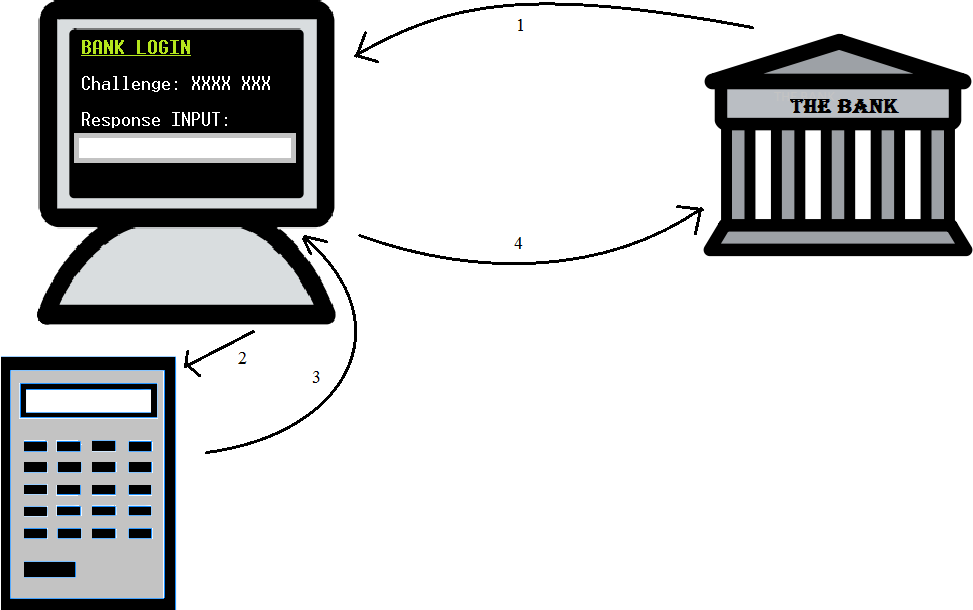
\includegraphics[scale=0.3]{img/challenge-response-bank}
    \caption{Challenge-response authentication with bank card reader}
  \label{fig:challengeResponse}
\end{figure}
Describing of~\figureref{fig:challengeResponse}:
\begin{enumerate}
	\item Bank sending Challenge XXXX XXX to the requesting address.
	\item User enter PIN and XXX XXX in the bank card reader.
	\item The reader encrypts the PIN and number with a secret key shared with the bank. The first numbers of the encryption is displayed o the reader. ($YYYY YYY = {XXXX XXX, PIN}_k$) 
	\item The user enter the encrypted numbers YYYY YYY on the log in screen and sends it as a password to the bank.
\end{enumerate}
~\cite[ch.3]{rosssec}

\section{M2M\index{M2M} (Machine-to-machine)}\label{sec:m2mauth}
Information that is exchanged via a communication network between machines has to establish conditions for doing so, that is where M2M is used. M2M is often a short synonym for M2M communication, meaning the communication conditions between devices. M2M communication is only the communication made between machines without any human behind it. A mobile device interacting with a call center application is not M2M, cause there is a human behind the mobile device calling. The reason for that using mobile devices in this thesis is that they have many hardware parts that can be used for no human communication with other devices (see chapter ~\ref{cha:character}). These hardware parts can be found in other simpler devices such as accelerometer sensor probe that also can be applied on the result.
\\
Often is M2M involving similar devices  in the same M2M area network, interacting with an application. This makes it possible for devices to access public networks as well, via a gateway or router. An example is the heating system in smart homes. 
Devices are not a new thing, but when we have a growing world of IoT devices with very specific characteristics is growing. Thus makes the area of M2M more important to make these devises talk without a human behind. This affecting the requirements on the application and networks dealing with the devices. Characteristics of this devices is listed blow;
\begin{itemize}
	\item[] \textbf{Multitude}, they say that connected devise not directly interacting with humans, the big part of IoT is soon to be significant more than the ones which interact directly with humans. This will put more pressure on application and networks dealing with all devices.
	\item[] \textbf{Variety} of connected devices with requirements like data exchange rate, form factor, computing, or communication capabilities. M2M applications have to be built, in order to define and develop common enabling capabilities.
	\item[] \textbf{Invisibility} meaning that the device has virtually zero human control. The more invisibly the less likely for error caused by humans. 
	\item[] \textbf{Criticality} devices that can harm humans like voltage. Therefor reliability is an important factor. 
	\item[] \textbf{Intrusiveness} many of the increasing connected devices raise the privacy question like refrigerators, stoves, doors, etc.
\end{itemize}
All this devices with no human control is like told above very different, but many of them is similar in some ways, such that the functionality is limited, low-powered, embedded and have long life cycles. The fact that they often are embedded makes it hard to separate between M2M communication and machine-to-human or human-to-human communication.
\cite[p.~2-4]{m2mComm}

\subsection{Difference between M2M and IoT}
Internet-of-Things, meaning to making everything connected to everything in the Internet. IoT is now in its starting pits and ready to start the race. Machine-to-machine communication is a part of that, but it also covers other areas and IoT some that M2M doesn't. The common denominator is according to Polsonetti \textit{remote device access}, where the embedded hardware modules in a machine that communicate wireless or not is M2M applications. Remote device access for IoT has a much more wider perspective that not only including same device communication but also passive and other low-power sensors that not can be motivated as a M2M hardware module.
\cite[]{cpM2MIoT}\\
In this thesis is M2M a subset of IoT, since it always one mobile device that wants to authenticate then it can communicate with other deceives.

\subsection{M2M authentication}
There are no standardized way of authenticate in M2M, but effort is done in the area. An example is \cite[]{auth:M2M} where he based authentication on a machines fingerprint. But this fingerprint isn't of the same character as the one this thesis is focusing on. In his article the fingerprint consist of hardware message of computers, such serial number of CPU, MAC address of network card, Machine ID etc. These things have through the years been proven to bee pretty easy to spoof. There are hundreds of guides on blogs and forums of how to do that in many platforms like mobile devices. \\
\\
Like \cite[]{auth:M2Mcom} that states in their article that ``\dots traditional methods such as “what you know and who you are” may not be applied''. As stated in the aim of the thesis  (section~\ref{sec:aim}) is to do precisely that and with the advantage that using ``regular'' authentication that is more  tried and tested. Thus the next section will be about biometric systems and how they authentication which is used for who you are.


\section{The biometric process}\label{sec:biometric}
\begin{center}\textit{``A biometric system measures one or more behavioral characteristics...information of an individual to determine or verify his identity.''} \cite[p.~3]{introbio}\end{center}

\subsection{Recognition}
As said before is biometric something you \textit{are} and the person who wants to be recognized to the system. Buy, showing his or her biometric identifier (fingerprint, iris, DNA, etc.) to the biometric system, thus seen as a \textit{user} of the system. The strength in biometrics is also the fact that it knows if a user is known to the system even if the user denies it. \cite[ch.~1]{introbio}

\subsection{Biometric systems}
There are some blocks for building a biometric systems, which can measure characteristics of a user. In biometric these characteristics is called \textit{traits, indicators, identifiers, or modalities}, but for for the aim of this thesis will it still be called characteristics. For designing, implementation and evaluation when building a biometric system there are some steps that has to be done;\\
\\
The first step is to collect biometric data and store it in a database with the users identity. The recognition is then done by again collect biometric data from the user and compared to the database. This is the so called \textit{enrollment and recognition phase}. The raw biometric data is often destroyed after enrollment and the recognition is all about pattern matching. This matching is done in four steps;
\begin{enumerate}
	\item \textit{Sensor -} to collect the raw biometric samples, that can be a image, amplitude signal, online signature, odor or chemical-based.
	\item \textit{Feature extractor -} first has to make the raw biometric samples comparable, mostly done in three pre-process operations; 
	\begin{itemize}
    	\item Quality assessment, is the sample good enough?
		\item Segmentation, remove background noise from sample
		\item Enhancement, by using an algorithm to improve the sample 
    \end{itemize}
	\item \textit{Database -} that has the data from the enrollment phase together with some identity data (like name orID). This database should having a access control mechanism for security reasons.
	\item \textit{Matcher -} where the sample from the enrollment is compared with the sample in recognition, to see if it's a match or not. This is done by having a match score to decide how close the enrolled and recognition sample is. The score is counted in different way depending on the characteristics that is used in the system. 
\end{enumerate}
\cite[ch.~1]{introbio}

\subsection{Biometric authentication}
Biometrics authentication, is sometimes also called verification that answers the question ``Are you the one you say you are?''. There is also biometric identification that answers ``Are you someone known to the system?'' but that is not what this thesis aim to answer. The practical difference between authentication and identification is that the user has to give the system some kind of information (username, passport, email etc.) on who they claim to be. But in identification the user just give the sample to the system, which then looks if the user is known to the system or not. The identification look-up takes longer time since you look for all samples in the database and compare them, in authentication you only look for the claimed identity. \cite[ch.~1]{introbio}

\subsection{Measurements}\label{sec:bio:measure}
Biometric measurements is a bit more tricky than in a password-based system where the answer just is `match' or `no match'. The accuracy of the biometric system must be consider when you choose characteristics. This is measured by two rates \index{FRR} (False Reject Rate) that is the probability that two samples from the same user is not a match and \index{FAR} (False Accept Rate) is the probability that two samples from different users is a match. A match is decided authentic between two samples from the same user is high enough and as a \textit{impostor} is there is similarity between two samples from different users.  \\
There are a threshold $\eta$ that is used to decide the FRR and FAR. The proportion of authentic scores ($\omega_{1})$) that are less than $\eta$ is defined as FRR and the impostor score ($\omega_{0})$) that are greater than or equal to $\eta$ is FAR. Which can be described mathematical as; 
$$ FAR(\eta) = p(s\geq \eta | \omega_{0}) = \int_{\eta}^{\infty} p(s | \omega_{0}) ds, $$
$$ FRR(\eta) = p(s\geq \eta | \omega_{1}) = \int_{-\infty}^{\eta} p(s | \omega_{1}) ds, $$
where $p(s\geq \eta | \omega_{x})$ us the probability density function of the authentic respective impostor score. 
\cite[p.~18]{introbio}

\subsection{Design a biometric system}
When designing a biometric system it is done in a five activity cycle. Depending on the outcome of one activity, the next step could be forward or redoing earlier activity. The design cycle is represented as a flow-chart below (from page 27 in \cite[]{introbio}), followed by a description of the five activities. \\
\\
\textbf{Understand nature of application -} is about deciding functionality type and classified based on how well the system fits this six different behaviors; cooperative, overt, habituated users, attended, untenanted operation, controlled operation and open system. The first is if the user will be \textit{cooperative} or not, like if the user wants to access something it is likely to cooperate. \textit{Overt} is if the user knows that it is object for biometric recognition. If the user interacts with the system a lot it is likely that the user will be \textit{habituated}. The enrollment and recognition operations can either be \textit{attended} by a human or not. The environment of the operations may have to be \textit{controlled} in terms of temperature, pressure, etc. in order to work. Last there are also the question if the system will be closed or \textit{open}, such if the database of biometric data will be shared between applications or be in one closed application.) \\
\\
\textbf{Choose biometric characteristics -}\label{auth:bio:character} is also classified, based on seven different factors. The thing with biometrics is that it will never be completely solid, thus all the factors can't be perfect. Counted to this is that the factors will have different value for different systems.
\begin{enumerate}
	\item \textit{Universality,} the fail-to-enrollment (FTE) rate should be low.
	\item If the \textit{uniqueness} of the characteristics is high will the rate of FAR be low. 
	\item The characteristic should be high in terms of \textit{permanence} and not be changing significantly over time.
	\item \textit{Measurability} from the user perspective in terms of collecting characteristics, should convenient.
	\item The time of the authentication is measured in \textit{performance}.
	\item User should have a high \textit{acceptability} in present their characteristics to the system.
	\item \textit{Circumvention}, in terms of how easy it is to malicious fake the characteristics.
\end{enumerate} 

\textbf{Collect biometric data -} is apart from the collecting also includes factors of time, cost and size of the equipment.\\
\\
\textbf{Choose features and matching algorithm -} is a critical step since this is the heart of the system and has to bee done with a great deal of knowledge if the selected characteristics and the data extracted from it. \\
\\
\textbf{Evaluate the biometric system -} by asking different questions. There are no framework for doing this and it has to account different perspective as require experts of different field such psychology, business, computer science and statistics. There exists no framework for these types of evaluation but \cite[]{introbio} propose doing it in three evaluation-stages technology, scenario and operational.

\begin{figure}[!ht]
	\begin{tikzpicture}[node distance=1.6cm]
	\node (start) [justtext] {Start};
	\node (understand) [process, below of=start] {Understand nature of application};
	\draw [arrow] (start) -- (understand);
		
	\node (choose) [process, below of=understand] {Choose biometric characteristics};
	\draw [arrow] (understand) -- (choose);
		
	\node (collect) [process, below of=choose] {Collect biometric data};
	\draw [arrow] (choose) -- (collect);
	\node (coll) [right of=collect, xshift=1.3cm] {};

	\node (algorithm) [process, below of=collect] {Choose features and matching algorithm};
	\draw [arrow] (collect) -- (algorithm);
	\node (alg) [right of=algorithm, xshift=1.3cm] {};

	\node (evaluate) [process, below of=algorithm] {Evaluate the biometric system};
	\draw [arrow] (algorithm) -- (evaluate);

	\node (end) [justtext, below of=evaluate] {End};
	\draw [arrow] (evaluate) -- (end);

	\node (req) [justtext, text=blue, left of=understand, xshift=-3cm, yshift=-1cm] {Performance requirements};
	\draw (understand) -| (req);
	\draw [->,>=stealth] (req) |- (evaluate);
		
	\node (knowledge) [justtext, text=red, left of=algorithm, xshift=-1.5cm] {Prior knowledge};

	\draw [arrow, draw=red, very thick] (knowledge) |- (algorithm);

	\draw [dashed] (evaluate) -| (alg);
	\draw [darrow, dashed] (alg) -- (algorithm);
	\draw [dashed] (alg) -- (coll);
	\draw [darrow] (coll) -- (collect);
	\draw [darrow] (coll) |- (choose);
\end{tikzpicture}
	\caption{\label{fig:biodesigncycle} The design cycle of a biometric system}
\end{figure}
\chapter{HARDWARE CHARACTERISTICS OF A MOBILE DEVICE}\label{cha:character}\index{characteristics}
In the hardware of a device there are some features that can be used to distinguish devices from each other. In most cases it is not called features rather error sources. In the aim of this thesis it is feature characteristics that can be seen as an uniqueness of an mobile device. \textit{Device fingerprint(ing)}\index{device fingerprint} is the term used for this feature characteristics and the pyramid seen in~\figureref{fig:pyramid} from ~\cite[]{sensor:acoustic} shows the different types of sources of device fingerprint. This thesis will focus on the top of quarter of that pyramid, that is the sensors. All error sources of sensors comes in form of bias and the bias from each sensor covered by the thesis is further explained in this chapter. There is also an explanation on how the sensors is measured from Android respective JavaScript depending on the preformed tests that is described in ~\chapterref{cha:measurements}.

\begin{figure}[!h]
		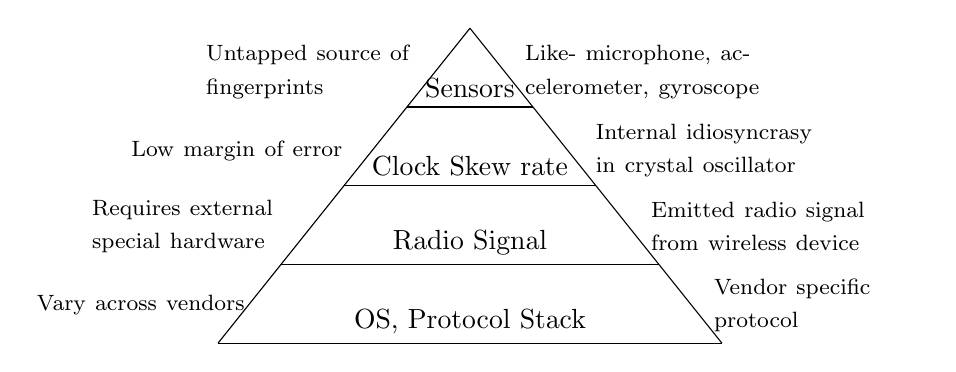
\begin{tikzpicture}[scale=1]

		\def \h {4};
		\def \f {0.8};

		\foreach \y in  {0,1,2,3} {
		    \def \w { \h*\f-\y*\f };
		    \def \v { \y*\f-\h*\f };
		    \draw (\v,\y) -- (\w,\y);
		}

		\draw (-\h*\f,0)  -- (0,\h);
		\draw (\h*\f,0)  -- (0,\h);
		\node (os) at (0,0) [above] {OS, Protocol Stack};
		\node (rf) at (0,1) [above] {Radio Signal};
		\node (cs) at (0,2) [above] {Clock Skew rate};
		\node (se) at (0,3) [above] {Sensors};


		\node [left of=os, xshift=-3cm, yshift=0.2cm, text width=3cm] {\footnotesize{Vary across vendors}};
		\node [left of=rf, xshift=-2.4cm, yshift=0.2cm, text width=2.8cm] {\footnotesize{Requires external special hardware}};
		\node [left of=cs, xshift=-1.8cm, yshift=0.2cm, text width=3cm] {\footnotesize{Low margin of error}};
		\node [left of=se, xshift=-1cm, yshift=0.2cm, text width=2.7cm] {\footnotesize{Untapped source of fingerprints}};

		\node [right of=os, xshift=3.4cm, yshift=0.2cm, text width=2.6cm] {\footnotesize{Vendor specific protocol}};
		\node [right of=rf, xshift=2.8cm, yshift=0.2cm, text width=3cm] {\footnotesize{Emitted radio signal from wireless device}};
		\node [right of=cs, xshift=2.1cm, yshift=0.2cm, text width=3cm] {\footnotesize{Internal idiosyncrasy in crystal oscillator}};
		\node [right of=se, xshift=1.3cm, yshift=0.2cm, text width=3.2cm] {\footnotesize{Like- microphone, accelerometer, gyroscope}};
	\end{tikzpicture}
	\caption{\label{fig:pyramid} The pyramid of features in a mobile device that can be used for fingerprinting.\cite[]{sensor:acoustic}}
\end{figure}

As seen above in~\figureref{fig:pyramid} are sensors an untapped source of fingerprints in mobile devices and example of sensors are microphone, accelerometer, barometer, speakers and gyroscope. The sensors investigated in this work is the accelerometer-, gyroscope-, magnetometer- and camera- sensors. All of them are common sensors in most of the mobile devices used today.


\section{Accelerometer\index{accelerometer}}\label{sec:accelerometer}
The accelerometer is the sensor that detect movement on a mobile device, like when you changing orientation on your device. Acceleration is measured by sensing how much pressure the device has in terms of force. The type of accelerometer sensor found in a mobile device is a micro-electromechanical systems known as MEMS sensor. \cite[]{sensors:fusion}
\subsection{Fingerprinting feature / Bias}
Measure the characteristics from the accelerometer is done by taking the long term average of the output when the accelerometer is in rest. That is the biggest error source in the accelerometer and it grows quadratically over time, but when the accelerometer is in rest the error $\epsilon$ can be calculated as a function of time $t$;
\begin{equation} \label{eq:AccBias}
s(t)=\epsilon * \frac{t^2}{2} 
\end{equation}
\cite[]{sensor:inertialNav}\cite[]{sensors:fusion}


\section{Gyroscope\index{gyroscope}}\label{sec:gyroscope}
The gyroscope is sensing how the device is moving in terms of angles, for maintaining or measure the orientation. This is originally  a mechanical system based on the principle of conservation of angular momentum. The most popular Gyroscope for devices today is a MEMS that is using silicon micro-mechanical techniques. Coriolis effect is measured with vibrating elements in the MEMS gyroscope. Coriolis effect is a change of moving objects direction when looking at it from a rotating reference system. The difference from the accelerometer is that the gyroscope measures relative to the device body rather than relative to earth. The equations of Coriolis force;  
$$\boldsymbol{ F}_C = -2 \, m \, (\omega *  v)$$
Where $m$ is the mass of the particle, $\omega$ the angular velocity and $v$ the velocity of the particle in the rotating system. 
\cite[]{sensor:inertialNav}
\subsection{Fingerprinting feature / Bias}
The gyroscope has some error characteristics like constant bias, white noise, bias instability, calibration error and temperature effects. One of these error characteristics that can be tested by reading the output from a gyroscope in rest is the \textit{constant bias}\index{constant bias}. That is bias of the gyroscope output when not having any rotation on it. This constant error $\epsilon$ of the bias over time $t$ leads to an angular error that grows linear; 
\begin{equation} \label{eq:gyroBias}
\theta (t)= \epsilon * t
\end{equation}
If take the long term average output from the gyro in rest, the constant error of a rate gyro can be estimated.\cite[]{sensors:fusion}


\section{Magnetometer\index{magnetometer}}
The magnetometer measures the magnetic field and was originally used for navigation and tracking. When it is used as a compass the Earth's magnetic field is measured. The type of sensor found in mobile devices is like accelerometer and gyroscope a MEMS sensor. They are known as e-compasses gaussmeters that is measuring of magnetic fields larger than 1 nT.
~\cite[]{sensor:magn}

\subsection{Fingerprinting feature / Bias}
\textit{Note that normally bias in a magnetometer is called \textbf{offset} but for uniformity reason of this report it will be referenced to \textbf{bias}.}\\
\\
When try to measure the magnetic field of Earth with a magnetometer it also gets affected by other magnetic fields. The two main error sources from measurements of magnetometer are magnetic contamination in the sensor, called Soft and Hard-Iron distortion. \\
The hard iron distortion is caused by metals and magnets around the magnetometer. This field is constant even if the device moves, thus it is additive to the earths magnetic field. This distortion can be caused of e.g. the device speaker mounted near the magnetometer. \\
If there are magnetic fields in the surrounding environment of the device they will cause soft iron disorder. This error is smaller than the hard iron distortion. Any metal around the device can cause this error, such a car passing by.
There are also a third bias that can effect the magnetometer and is as the hard iron distortion additive. This bias is the errors in the magnetometer itself such that all hardware has. But the result of this bias is similar to the soft iron distortion.  \\
The good thing with magnetometer bias is that it is constant over time, thus once it is calculated it stays the same. \\
\\
If the device is rotated one turn (360\degree)around its own z-axes (see~\figureref{fig:device-axes}) and plot x with respect to y there will be a circle. In a world without bias this circle will look like:
\begin{figure}[H]
\begin{tabular}{p{0.23\textwidth} p{0.23\textwidth} p{0.23\textwidth} p{0.23\textwidth}}
        \vspace{0pt} \begin{tikzpicture}[line cap=round,line join=round,>=triangle 45,x=1.0cm,y=1.0cm]
\draw[->,color=black] (-1.5,0.) -- (1.5,0.);
\foreach \x in {-1.4,-1.2,-1.,-0.8,-0.6,-0.4,-0.2,0.2,0.4,0.6,0.8,1.,1.2,1.4}
\draw[shift={(\x,0)},color=black] (0pt,-2pt);
\draw[color=black] (1.3548383992423667,0.012646598999199708) node [anchor=south west] {X};
\draw[->,color=black] (0.,-1.5) -- (0.,1.5);
\foreach \y in {-1.4,-1.2,-1.,-0.8,-0.6,-0.4,-0.2,0.2,0.4,0.6,0.8,1.,1.2,1.4}
\draw[shift={(0,\y)},color=black] (-2pt,0pt);
\draw[color=black] (0.015808248748999637,1.4306334471160802) node [anchor=west] {Y};
\clip(-1.5,-1.5) rectangle (1.5,1.5);
\draw(0.,0.) circle (1.cm);
\begin{scriptsize}
\draw [color=xdxdff] (0.,0.)-- ++(-2.0pt,-2.0pt) -- ++(4.0pt,4.0pt) ++(-4.0pt,0) -- ++(4.0pt,-4.0pt);
\draw [fill=qqqqff] (0.,1.) circle (1.5pt);
\draw[color=qqqqff] (-0.15,1.1) node {0\textrm{\degre}};
\end{scriptsize}
\end{tikzpicture}
 & 
        \vspace{0pt} \begin{tikzpicture}[line cap=round,line join=round,>=triangle 45,x=1.0cm,y=1.0cm]
\draw[->,color=black] (-1.5,0.) -- (1.5,0.);
\foreach \x in {-1.4,-1.2,-1.,-0.8,-0.6,-0.4,-0.2,0.2,0.4,0.6,0.8,1.,1.2,1.4}
\draw[shift={(\x,0)},color=black] (0pt,-2pt);
\draw[color=black] (1.3548383992423672,0.012646598999199708) node [anchor=south west] {X};
\draw[->,color=black] (0.,-1.5) -- (0.,1.5);
\foreach \y in {-1.4,-1.2,-1.,-0.8,-0.6,-0.4,-0.2,0.2,0.4,0.6,0.8,1.,1.2,1.4}
\draw[shift={(0,\y)},color=black] (-2pt,0pt);
\draw[color=black] (0.015808248748999637,1.4306334471160802) node [anchor=west] {Y};
\clip(-1.5,-1.5) rectangle (1.5,1.5);
\draw(-0.2,-0.2) circle (1.003958800671448cm);
\begin{scriptsize}
\draw [fill=qqqqff] (-0.18558461983368865,0.8038553034478191) circle (1.5pt);
\draw[color=qqqqff] (-0.16,1) node {0\textrm{\degre}};
\draw [color=xdxdff] (-0.2,-0.2)-- ++(-2.0pt,-2.0pt) -- ++(4.0pt,4.0pt) ++(-4.0pt,0) -- ++(4.0pt,-4.0pt);
\end{scriptsize}
\end{tikzpicture} & 
        \vspace{0pt} \begin{tikzpicture}[line cap=round,line join=round,>=triangle 45,x=1.0cm,y=1.0cm]
\draw[->,color=black] (-1.5002742877331638,0.) -- (1.5002742877331638,0.);
\foreach \x in {-1.4,-1.2,-1.,-0.8,-0.6,-0.4,-0.2,0.2,0.4,0.6,0.8,1.,1.2,1.4}
\draw[shift={(\x,0)},color=black] (0pt,-2pt);
\draw[color=black] (1.3548383992423672,0.012646598999199708) node [anchor=south west] {X};
\draw[->,color=black] (0.,-1.500215870948452) -- (0.,1.5001897416116785);
\foreach \y in {-1.4,-1.2,-1.,-0.8,-0.6,-0.4,-0.2,0.2,0.4,0.6,0.8,1.,1.2,1.4}
\draw[shift={(0,\y)},color=black] (-2pt,0pt);
\draw[color=black] (0.015808248748999637,1.4306334471160802) node [anchor=west] {Y};
\clip(-1.5002742877331638,-1.500215870948452) rectangle (1.5002742877331638,1.5001897416116785);
\draw [rotate around={-36.86989764584405:(0.,-0.15)}] (0.,-0.15) ellipse (1.1608455676650522cm and 0.8860374890305703cm);
\begin{scriptsize}
\draw [color=xdxdff] (0.04907705257499707,-0.12173658003568395)-- ++(-2.0pt,-2.0pt) -- ++(4.0pt,4.0pt) ++(-4.0pt,0) -- ++(4.0pt,-4.0pt);
\draw [fill=qqqqff] (-0.8962562226151813,0.5864729639194997) circle (1.5pt);
\draw[color=qqqqff] (-1.1,0.75) node {0\textrm{\degre}};
\end{scriptsize}
\end{tikzpicture} & 
        \vspace{0pt} \begin{tikzpicture}[line cap=round,line join=round,>=triangle 45,x=1.0cm,y=1.0cm]
\draw[->,color=black] (-1.500130470417328,0.) -- (1.5002743955178048,0.);
\foreach \x in {-1.4,-1.2,-1.,-0.8,-0.6,-0.4,-0.2,0.2,0.4,0.6,0.8,1.,1.2,1.4}
\draw[shift={(\x,0)},color=black] (0pt,-2pt);
\draw[color=black] (1.3548385432174719,0.012646598999199708) node [anchor=south west] {X};
\draw[->,color=black] (0.,-1.500215870948452) -- (0.,1.5001897416116785);
\foreach \y in {-1.4,-1.2,-1.,-0.8,-0.6,-0.4,-0.2,0.2,0.4,0.6,0.8,1.,1.2,1.4}
\draw[shift={(0,\y)},color=black]  (-2pt,0pt);
\draw[color=black] (0.015808244815253596,1.4306334471160802) node [anchor=west] {Y};
\clip(-1.500130470417328,-1.500215870948452) rectangle (1.5002743955178048,1.5001897416116785);
\draw [rotate around={0.059845574260994405:(4.8164851529053886E-4,7.838801032565946E-4)}] (4.8164851529053886E-4,7.838801032565946E-4) ellipse (1.2496624710485813cm and 0.9992161789727994cm);
\begin{scriptsize}
\draw [color=xdxdff] (0.,0.)-- ++(-2.0pt,-2.0pt) -- ++(4.0pt,4.0pt) ++(-4.0pt,0) -- ++(4.0pt,-4.0pt);
\draw [fill=qqqqff] (0.,1.) circle (1.5pt);
\draw[color=qqqqff] (-0.15,1.1) node {0\textrm{\degre}};
\end{scriptsize}
\end{tikzpicture} \\
        \vspace{0pt} Ideal & Hard Iron distortion & Soft Iron distortion & Gain mismatch \\
\end{tabular}
\caption{Example of different magnetometer readings when affected by bias.}\label{fig:magnCircle}
\end{figure}
\cite[]{liu:magnAcc}

\subsection{Magnetometer calibration}
To do a magnetometer calibration the device is turned 360\degree around the z-axis (~\figureref{fig:device-axes}), with the device on a flat surface. This makes x and y-axis the surface and z-axis pointing (UP/DOWN?). To calculate the offset $O_{x,y,z}$ the average of min and max-value from each axis is calculated (the center of the circle) from the magnetic field $B_{x,y,z}$, like:
\begin{subequations}
\begin{align}
  O_x = \frac{max(B_x) + min(B_x)}{2} \\
  O_y = \frac{max(B_y) + min(B_y)}{2} \\
  O_z = \frac{max(B_z) + min(B_z)}{2}
\end{align} 
And the hard iron compensated result $m_{x,y,z}^h$:
\begin{align}
  m_x^h = B_x - O_x \\
  m_y^h = B_y - O_y \\
  m_z^h = B_z - O_z
\end{align}
\end{subequations}
The soft iron is sometimes compensated for in the equations above and sometimes additional compensation has to be done. Since soft iron offset is place specific it will not be considered in the thesis since a fingerprint of a device is not convenient if you have to be at the exact same spot every time the device tries to authenticate.
\cite[]{liu:magnAcc}


\section{Camera}\label{sec:char:camera}\index{camera fingerprinting}\index{camera}
\textit{Note that normally bias in a camera sensor is called \textbf{noise} but for uniformity reason of this report it will be referenced to \textbf{bias}.}\\
\\
The digital camera of a mobile device also includes sensors and other hardware that can be used as fingerprinting characteristics. The basic is that light travels trough a lens and hits a imaging sensor which contains pixels that has a filter array in front. The filter is for gives each pixel a detected color. The pixels is then put together again to a resulting signal which is send to some final post processing (color correction, white balance, etc.) steps before the image is written to the memory card. In this process there are different kind of bias that effects the image;
\begin{itemize}
	\item[] \textit{\index{shot noise}Shot noise -} the amount of photons hitting the sensor and each pixel varies a random amount
	\item[] \textit{\index{fixed pattern noise}Fixed pattern noise - }there is a small electric current that leaks from photo-diodes in each pixel, caused by dark current
	\item[] \textit{\index{photo-response non-uniformity noise}\index{PRNU}Photo-response non-uniformity noise (PRNU) -} is a bias that is not affected by temperature or humidity. When manufacturing sensors the silicon gets imperfection which causes that pixels aren't equally sensitive to light. This is the main source of pattern bias and makes it really unlikely for two cameras to have the same pattern.
\end{itemize}
The three types of bias can be described as a mathematical model for getting the output of the sensor $y_{ij}$:
$$y_{ij}=f_{ij}(x_{ij}+\eta_{ij})+c_{ij}+\epsilon_{ij}$$
where $f_{ij}$ is a multiple factor close to one that captures PRNU, $x_{ij}$ is the number of photons hitting the sensor, $\eta_{ij}$ the shot noise, $c_{ij}$ the dark current and $\epsilon_{ij}$ the additive random bias. The key for a unique fingerprint of the camera (in the mobile device) is to finding $f$.
\cite[]{sensor:camera:DCIdent}

\section{Previous work of device sensor fingerprinting}
Accelerometer fingerprinting is a recent field of studies compared to the camera fingerprint that had been around for a longer time. The camera has for a long time been an object of identification in forensic purposes and therefor many research has been made and are applied today. Most of them uses advanced algorithm to extract the fingerprint and time of extracting hasn't been a concern. However in the aim of authentication the process can't be to time-consuming. In the~\tableref{table:prevAcc} and~\tableref{table:prevCamera} previous studies is presented in brief, followed by a longer presentation. Studies of gyroscope fingerprinting haven't been found. The majority of recent studies regarding the gyroscope have been about speech recognition. \cite{sensor:speechGyro} 
\begin{table}[H]
\subsubsection*{Accelerometer}
\begin{tabular}{| p{1cm} | p{1cm} | p{2.5cm} | p{1.8cm} | p{3.5cm} |}
  Year & Devices & Purpose & Fingerprint & Ref. \\ \hline
  2014 & 107 & Identification & Statistics &~\cite{sensor:accelPrint} \\
  2014 & 3583 & Tracking & Bias offset &~\cite{sensor:micSpeak} \\
  This & 100 & Authentication & Statistics & This thesis \\ \hline
\end{tabular} 
\caption[Table caption text]{Comparing previous studies of accelerometer fingerprinting} \label{table:prevAcc}
\end{table}

\subsubsection*{\cite{sensor:accelPrint}: \textit{AccelPrint: Imperfections of Accelerometers Make Smartphones Trackable}}
This research shows that the accelerometer can be used in identification and tracking purposes of the device. It is performed on android devices with an android application and on stand alone accelerometer chips. Their fingerprint consists of statistics values of the recordings such mean, standard deviation, skewness, min and max-values in both time and frequency domain. The research makes recordings with and without vibrations and in different circumstances; in car, running, walking, standing still. Their test environment uses machine learning that uses the statistics to build a fingerprint.\\
The result is an accuracy on 98\% when having alien devices among the already known devices which. Alien devices means that they are not previous known for the system, e.g. separate new users from already register users. \\
The research also states that the time needed for identifying a device is 30 seconds and that CPU-load less than 40\% is not affecting the result. Another important thing to notice is that since the also used stand alone accelerometer in different OS it rule out the possibility of that an OS can affect the output from the accelerometer.~\cite[]{sensor:accelPrint}

\subsubsection*{\cite{sensor:micSpeak}: \textit{Mobile Device Identification via Sensor Fingerprinting}}
This research shows a much larger scale experiments of 3583 devices. Experiments are preformed using JavaScript in a web-page. The fingerprint consists of calculating the bias offset on the accelerometer data. The result however isn't as good as the previous with successful identification on 15.1\%. To improve the result UserAgent-data were added and success rate rises to 58.7\% but that is software-based identification that more easily can be modified at the client side.~\cite[]{sensor:micSpeak}\\
\\
Since the research is in such different sizes they are difficult to compare it may be the case that \textit{AccelPrint} gets similar success rate if scaling it up and vice versa. \\

\begin{table}[H]
\subsubsection*{Camera}
\begin{tabular}{| p{1cm} | p{1cm} | p{2.7cm} | p{3cm} | p{2.5cm} |}
  Year & Devices & Purpose & Fingerprint & Ref. \\ \hline
  2008 & 16 & Identification &  Probabilistic SVM classifier &~\cite{sensor:camera:blind} \\
  2009 & 150 & Identification & PRNU correlation &~\cite{sensor:camera:DCIdent} \\
  2014 & 20 & Authentication & PRNU correlation & This thesis \\ \hline
\end{tabular}
\caption[Table caption text]{Comparing previous studies of camera fingerprinting} \label{table:prevCamera}
\end{table}

\subsubsection*{\cite{sensor:camera:blind}: \textit{Blind Identification of Source Cell-Phone Model}}
Using a probabilistic SVM classifier based on different features they manage to get good result (success rate on 95.1\%) even on images that are manipulated such cropped, resized or rotated. This however is a small scale experiment with more advanced techniques that not can be applied in authentication purposes rather in forensics. The thing to notice here is that the experiment is preformed on cell-phones from 2008 when the pictures had less quality than todays smart-phones.~\cite[]{sensor:camera:blind}

\subsubsection*{\cite{sensor:camera:DCIdent}: \textit{Digital Camera Identification}}
One of the experiments performed in this research included 150 devices with images that had random motives, zoom and other post-processing. The fingerprint consisted of the PRNU correlation and resulted in a false reject rate on 2,4\% and a false acceptance rate on 0.043\%.~\cite[]{sensor:camera:DCIdent} \\
This research performed on digital cameras and can be relative fairly with tests performed on smart-phone cameras used today. Since the digital cameras of 2009 had around 11 mega-pixels, images size of 4000x3000 pixels, and digital zoom of 4 times and had HD video recording width 30 fps. Which is about the average smart-phones camera today.~\cite[]{gbg:kamera}
\chapter{TEST \& DESIGN}\label{cha:test}
In this chapter the methods used for testing the mobile devices for different characteristics is described. 

\section{Accelerometer \& Gyroscope}\label{sec:test:motion}
I decided to collect the data via a web-page since JavaScript can access gyroscope and accelerometer data without any permission or knowledge from the user \cite[]{sensor:DeviceOrientation:spec}. This only require that the device has Internet and a browser installed, no additional installations and completely cross-platform. \\
\begin{figure}[H]
  \hspace{-2cm}
  \centering
  \begin{minipage}[c]{.23\textwidth}
    \centering
    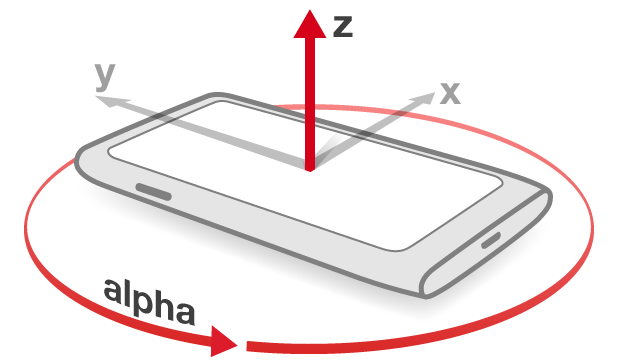
\includegraphics[scale=0.2]{img/device-alpha}
  \end{minipage}
  \hspace{1.5cm}
  \begin{minipage}[c]{.23\textwidth}
    \centering
    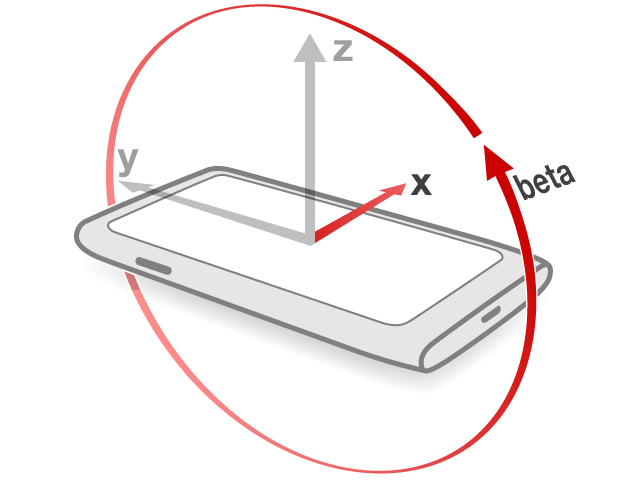
\includegraphics[scale=0.2]{img/device-beta}
  \end{minipage}
  \hspace{1.5cm}
  \begin{minipage}[c]{.23\textwidth}
    \centering
    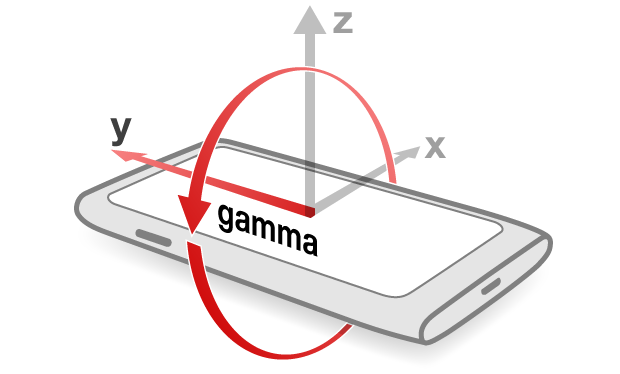
\includegraphics[scale=0.2]{img/device-gamma}
    \hspace{1cm}
  \end{minipage}
  \caption{The device axes for the JavaScript \texttt{DeviceOrientation} and \texttt{DeviceMotion}}
  \label{fig:device-axes}
\end{figure}

For the measurements of the accelerometer a event listener is added:
\lstinputlisting{code/acc-listener.js}
In JavaScript there are two types of acceleration with and without gravity, which according to Mozilla means that \texttt{accelerationIncludingGravity} is acceleration made by the device. In context to \texttt{acceleration} not depending on influence of gravity only by the acceleration made on the device. But as I see it that acceleration is made because of gravity so it is just different point of views. Since iOS has the z-axes pointed at the opposite direction that gives an additional security bit, that's why that one is used in this test. The accelerometer also comes with the nice feature of \texttt{rotationRate} which is the acceleration made from the axes in alpha, beta and gamma direction, see~\Figureref{fig:device-axes}. \cite[]{sensor:accIncludingGravity} \\
\\
For the measurements of the gyroscope another event listener is added:
\lstinputlisting{code/gyro-listener.js}
The \texttt{DeviceOrientation} is using the same axes as the accelerometer but the gyroscope is measuring how much the device is rotating along the \texttt{alpha, beta} and \texttt{gamma} axes in degrees (\Figureref{fig:device-axes}). The \texttt{alpha} is between 0 and 360 degrees, \texttt{beta} -180 to 180 degrees and \texttt{gamma} -90 to 90 degrees. \citet{sensor:DeviceOrientation:spec}.

\subsection{Accelerometer \& Gyroscope-test I}
The recording of the first accelerometer test is done by taking thousand accelerator-data samples during a few seconds and saved in a CSV for analyzing.
\begin{figure}[H]
  \hspace{-2cm}
  \centering
  \begin{minipage}[c]{.23\textwidth}
    \centering
    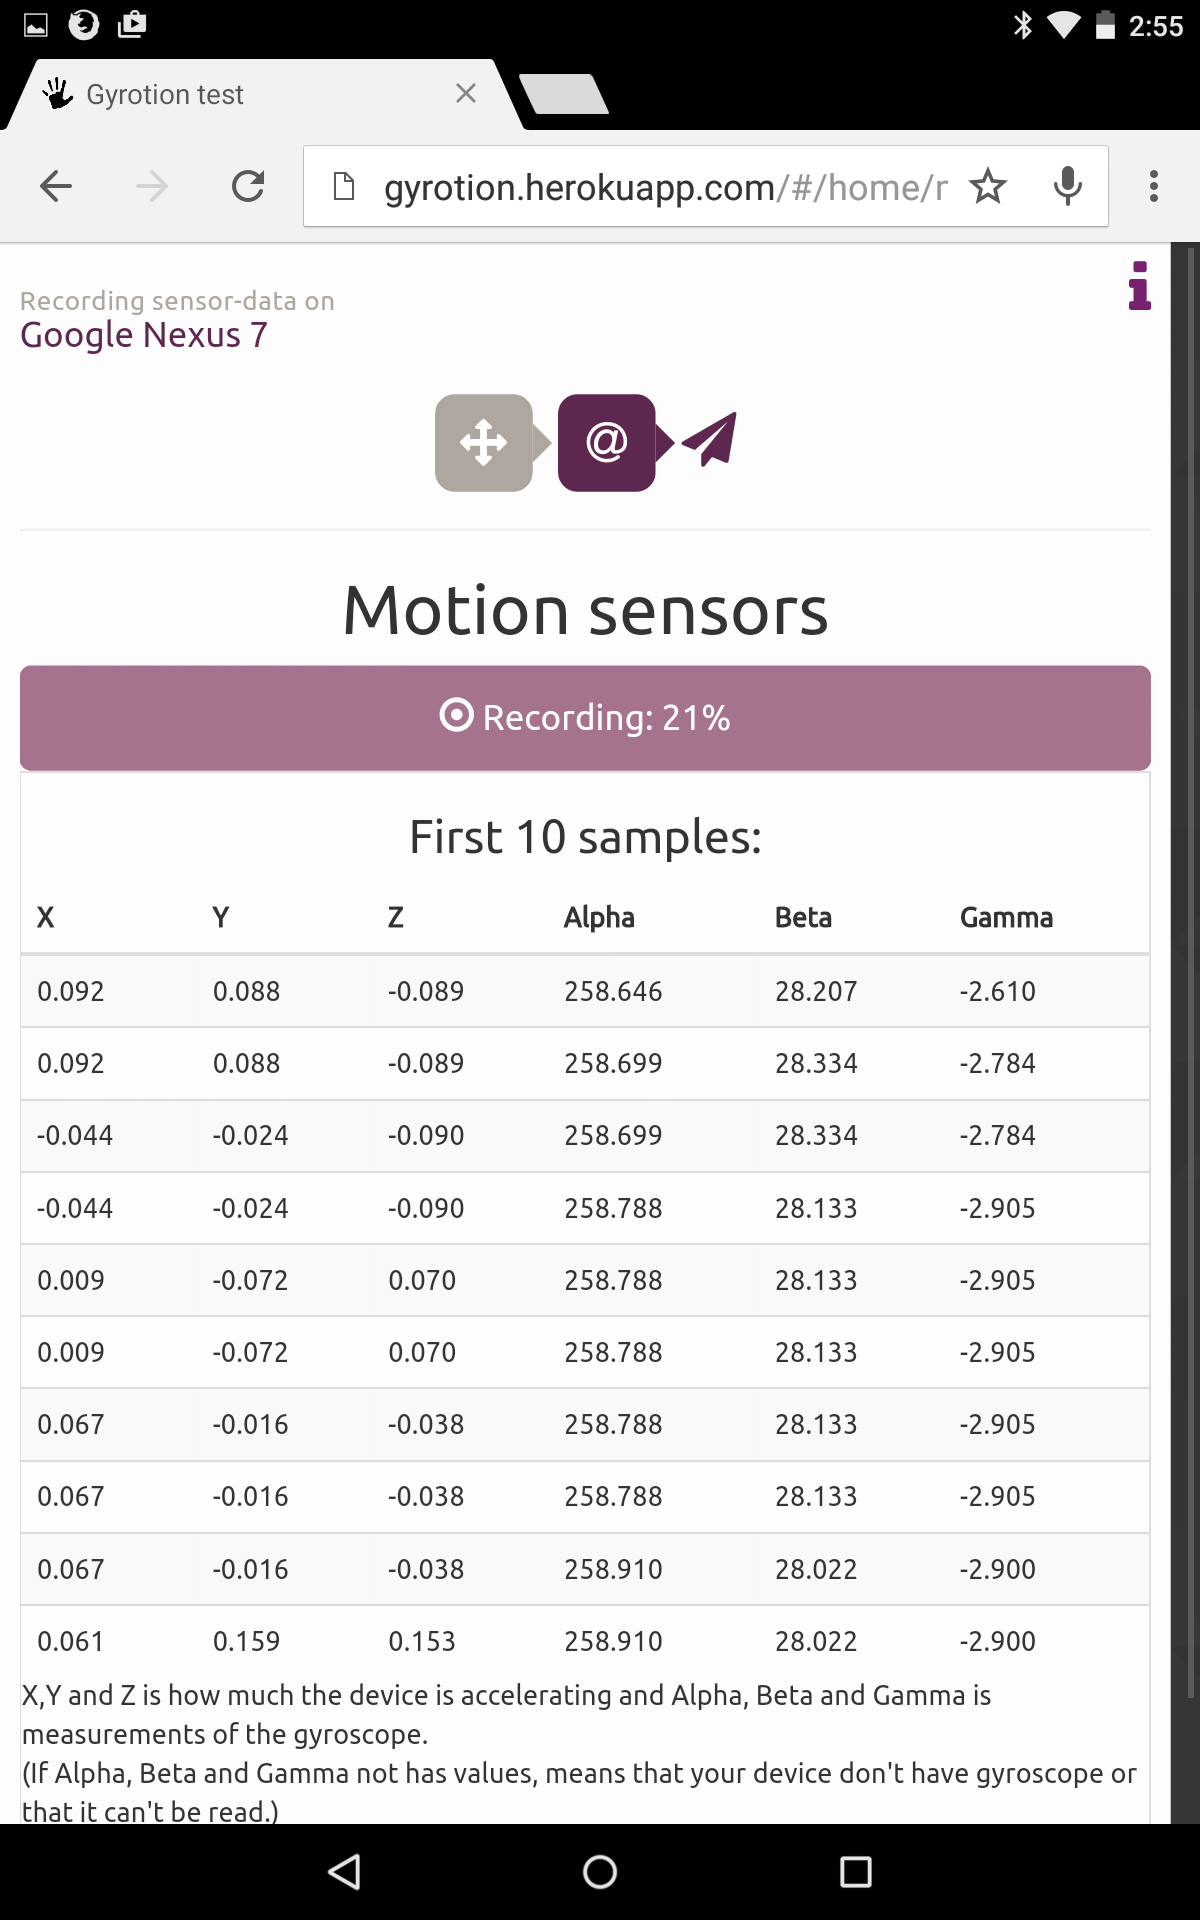
\includegraphics[scale=0.1]{img/Nexus-rec}
  \end{minipage}
  \hspace{2cm}
  \begin{minipage}[c]{.23\textwidth}
    \centering
    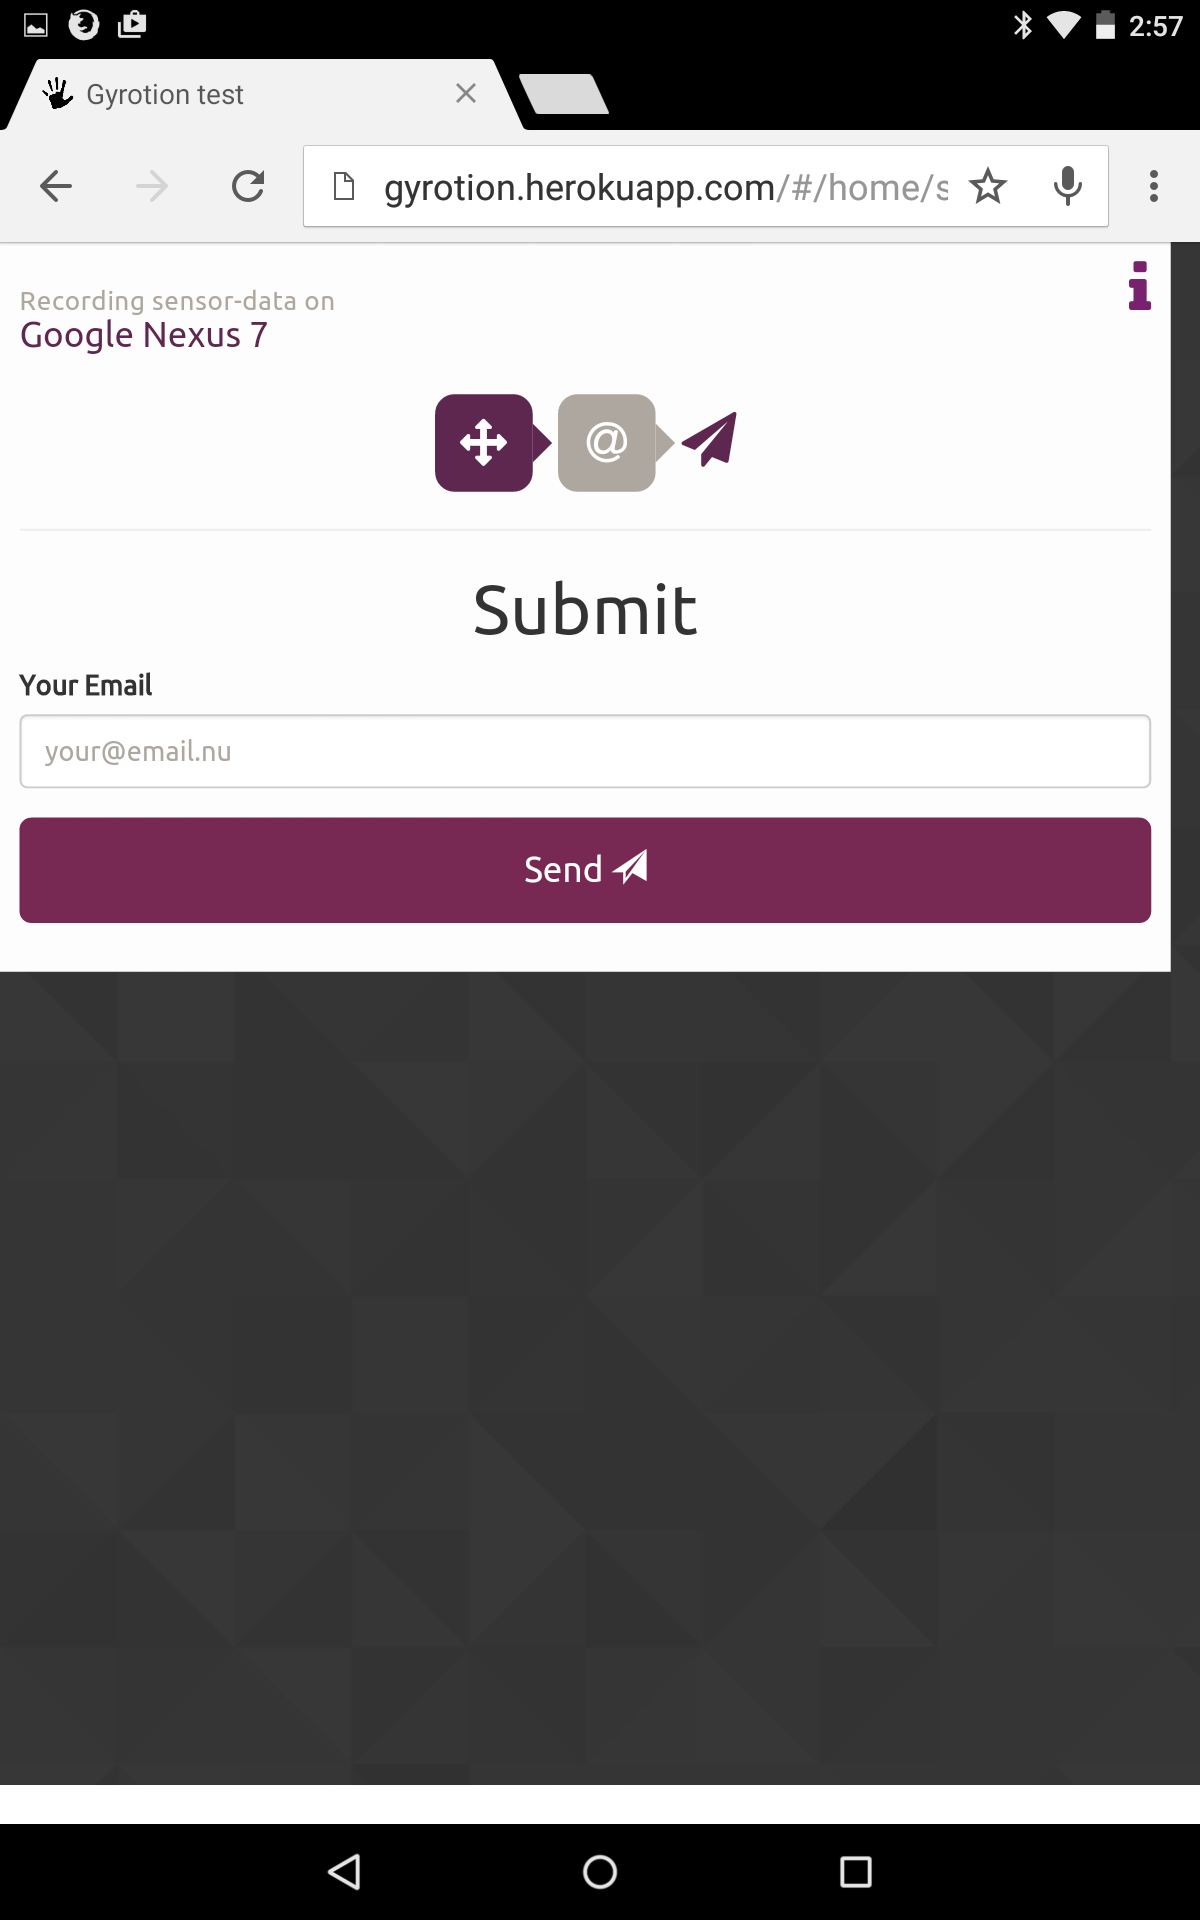
\includegraphics[scale=0.1]{img/Nexus-submit}
  \end{minipage}
  \caption{Screen shot from the page that  made recordings of accelerometer and gyroscope sensors in the first test}
  \label{fig:gyrotion}
\end{figure}

\subsection{Accelerometer \& Gyroscope-test II}
From the last test some changes were made to improve the test result:
\begin{itemize}
  \item Adding time-stamp to every recording sample to know exactly recording frequency
  \item Time based recording on 30 seconds instead of taking 1000 samples as in test I
  \item It's also sampling at a lower rate of at least 10 ms instead of as fast as it could before to reduce the effect of which other processes are in use on the device.
  % Ta bort ngn av pubkterna nedan?
  \item Make 2 recordings with the difference of a 180 degree rotation alpha wise (see \figureref{fig:device-axes}) for better bias estimation \cite{acc:kionixerr}.
  \item Added vibration in the recording to remove environmental noise which is one of the largest noise sources ~\cite[p.8]{acc:kionixerr} 
\end{itemize}

\section{Camera}\label{sec:test:camera}
For the test of the camera sensor the PRNU value is calculated as an approximation of the algorithm described in section ~\ref{sec:char:camera} and also used by \cite{sensor:camera:DCIdent}. That is the average of multiple image used and substantially an approximation of \textit{f}. The first step is to remove the image-content which leaves the noise, which is done using a denoising filter. For the test the MATLAB \texttt{medfilt2} is used, which is an 2-D median filtering that outputs the median value of each pixel by its 3-by-3 neighbors. 
\begin{figure}[H]
  \centering
  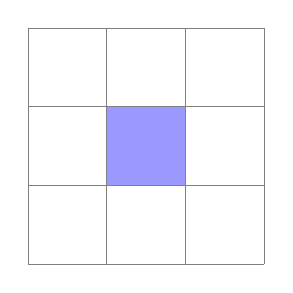
\begin{tikzpicture}[scale=1]
	\draw[step=1cm,gray,very thin] (0,0) grid (3,3);
	\fill[blue!40!white] (1,1) rectangle (2,2);
\end{tikzpicture}
  \caption{\label{fig:pyramid} the MATLAB \texttt{medfilt2} outputs the median of each pixel by it's 3-by-3 neighbors}
\end{figure}
From the \texttt{medfilt2} we gain a picture without noise which is then subtracted from the original to get the noise. This technique works best if there are no features on the image such auto-fix, black and white etc. The more images used for the average value the better noise is, thus the amount random noise is less and the fixed noise is more. \cite{sensor:camera:DCIdent} recommend a minimum of 50 images. This is then seen as the reference pattern used for correlating the noise from another image. This correlation is calculated like:
$$
corr(\boldsymbol{n},\boldsymbol{r}) = 
\frac{(\boldsymbol{n} - \bar{\boldsymbol{n}})(\boldsymbol{r} - \bar{\boldsymbol{r}})}
{\|\boldsymbol{n} - \bar{\boldsymbol{n}}\| \|\boldsymbol{r} - \bar{\boldsymbol{r}}\|}
$$
A threshold for acceptance on correlation is found by experimental on images taken with or without the camera. Then there is a balance between FAR and FRR. 

\section{Camera test I}
Since the purpose of this thesis compared to earlier work REFERENSER!! has the purpose of authentication and not forensics, is convenience for the collecting and measurability a factor to take in account. That is why the fist experiment is asked the users to record a 5 seconds video-clip with the device camera facing down on a flat object, like a table. Instead of making the user take 50 image or more which takes a lot of more time. This also makes it easier to get better noise since the same scene is used every time. \\
The video is then shuttled into images (100-200 from a 5 seconds video depending on fps on recording camera) that is used for calculating the PRNU. The MATLAB code for this is:\\
\rule{\textwidth}{0.5pt}
  \lstinputlisting{code/video2prnu1.m}
\rule{\textwidth}{0.5pt}

To compare an image between all collected PRNU the same calculation to get the noise is done. Then the noise from the reference image is compared to all collected PRNU and correlation is calculated like the formula above in MATLAB:\\
\rule{\textwidth}{0.5pt}
  \lstinputlisting{code/corrCamTest1.m}
\rule{\textwidth}{0.5pt}

\section{Camera test II}
Since the earlier test leaved out some of the PRNU noise when recorded a video instead of taking a picture the new test consist of 10 images from every device. The recommendation from \cite{sensor:camera:DCIdent} to use at least 50 images is here compensated by again using black images (picture taking with device camera facing down). Since the scene is always the same the noise removal will be better in fewer images. The same code is used as above with the different that the video to image step is removed. The sizes of the images in this case is better since the camera on the mobile devices by default uses higher resolution when taking a picture then when recording. 
\chapter{RESULT OF MEASUREMENTS}\label{cha:result}
This chapter covers the results of the measurements described in~\chapterref{cha:measurements}. The first two sections cover the measurements made on the accelerometer and gyroscope sensor. Third section cover the result of the two camera measurements.

\section{Pre-measurements}
To get a hint if accelerometer were a possible fingerprinting candidate some pre-measurements were preformed. This were in the early state of the development of the web-page used in measurements I and II. The measurement preformed on six different iPhones showed in~\figureref{fig:iPhoneScatter} indicates that the accelerometer is a sensor that may be good in fingerprinting purposes.
\begin{figure}[H]
\centering
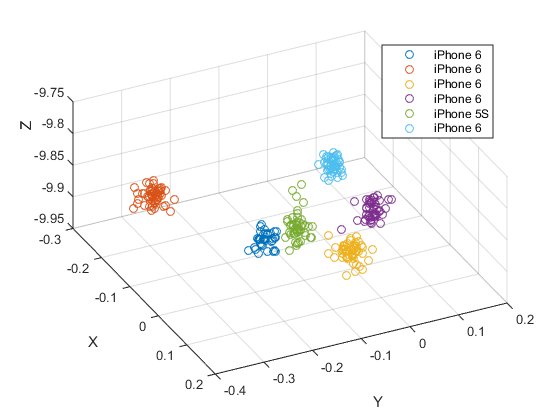
\includegraphics[scale=.6]{img/scatteriPhone}
\caption{Scatter-plot on accelerometer recordings of 6 Apple devices}
\label{fig:iPhoneScatter}
\end{figure}

\section{Result of measurements I  - Motion}\label{res:testI}
The data were gathered as described in~\sectionref{sec:measurementI} from the web-page in \figureref{fig:gyrotion} by spreading the the page. This resulted in over a hundred recordings, which had diversity in platforms, brands and models. Since the web-page where spread mostly to company employees the amount of devices with the same model is high as seen in ~\figureref{fig:measure1-topDevices}.
The purpose of this measurement where to identify if there where differences in terms of bias characteristics between the JavaScript's \texttt{accelerationIncludingGravity} and \texttt{acceleration}. The result of the measurements can be showed by making scatter-plots of the output acceleration of the devices. As shown in the ~\figureref{fig:measure1-topDevices} the \textit{Sony Xperia} devices represents more than a fifth of the total devices in the measurement. 
\begin{figure}[H]
	\centering
	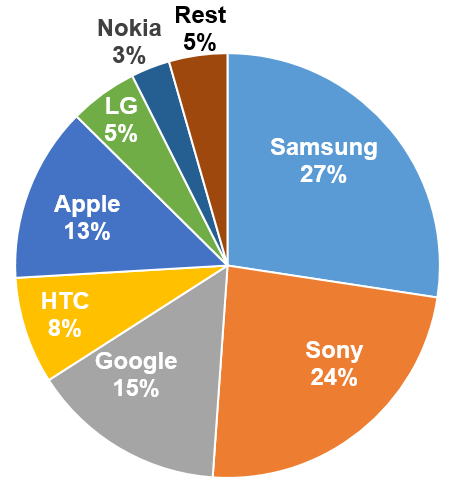
\includegraphics[scale=0.3]{img/measure1-brand}
	\caption{Diversity of device brand sampled in measurements I}
	\label{fig:measure1-brand}
\end{figure}
\begin{figure}[H]
	\centering
	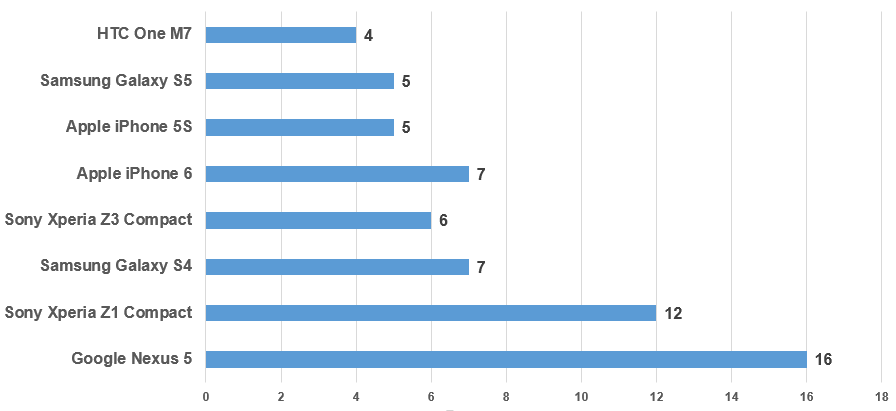
\includegraphics[scale=0.5]{img/measure1-devices}
	\caption{Most common devices models in measurements I}
	\label{fig:measure1-topDevices}
\end{figure}
The result of scatter-plots of measurements of 12 \textit{Sony Xperia} devices with and without gravity in accelerometer readings is shown in~\figureref{fig:scatter-withoutGrav} and~\figureref{fig:scatter-withGrav}.
\begin{figure}[H]
	\centering
	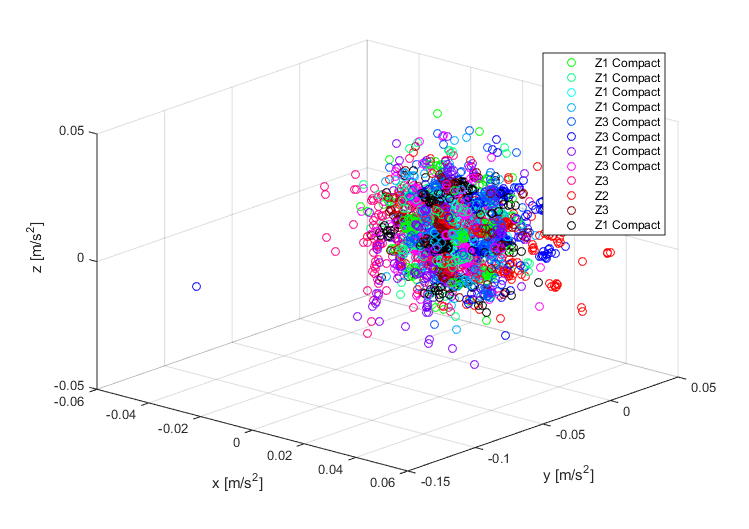
\includegraphics[scale=0.6]{img/res-measure1-scatter-notG}
	\caption{Bias from twelve \textit{Sony Xperia} deives measured with JavaScripts's \texttt{acceleration}}
	\label{fig:scatter-withoutGrav}
\end{figure}
\begin{figure}[H]
	\centering
	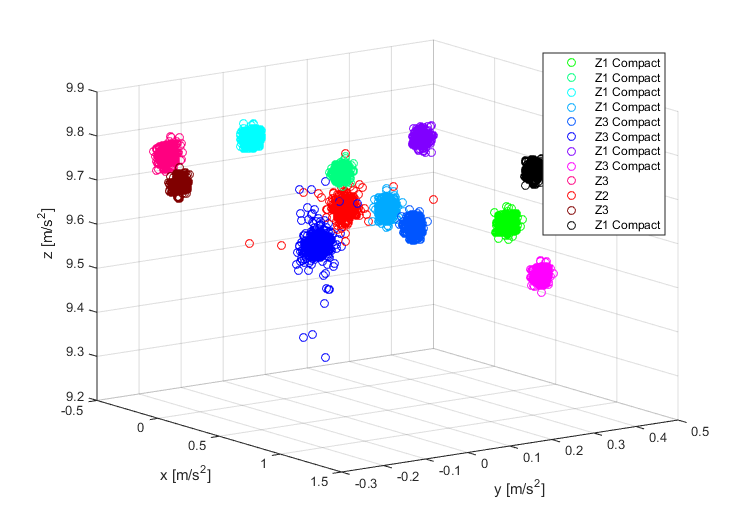
\includegraphics[scale=0.6]{img/res-measure1-scatter-inclG}
	\caption{Bias from twelve \textit{Sony Xperia} deives measured with JavaScripts's \texttt{accelerationIncludingGravity}}
	\label{fig:scatter-withGrav}
\end{figure}
As stated in~\cite{acc:kionixerr} the sources of bias in an accelerometer has to be compensated for. The manufacturer of the mobile devices makes some of this compensation before JavaScript gets the data. The results of the figures above indicates that JavaScript also makes compensating to the output of the event \texttt{acceleration}, probably to ease the development of software using the accelerometer, e.g. games. This however is not anything that is public in any specifications such~\cite{sensor:W3Cspec} or~\cite{sensor:accIncludingGravity}. The Android developer page about sensor event \cite{android:sensorEvent} state that they make factory calibration and temperature compensation even on their uncalibrated sensor events of (only magnetometer and gyroscope) that is relativity new feature added in Android 4.3 Jelly Bean (API level 18~\cite{android:API18}) from 2013 but the original once used since Android 1.5 Cupcake (API level 3~\cite{android:API3}) from 2009 makes some more noise compensation and calibration. What kind of compensation and calibration done is not public. 

\section{\textbf{Doing! }Result of measurements II  - Motion}\label{res:testII}
The result here is an analyses of the gyroscope and accelerometer data collected from 60 devices by an improved version of the JavaScript web-page used in measurements I. The changes that were made is described in~\sectionref{sec:measurementII} to improve that analyze data. \\
The diversity of the devices brands in the measurement is shown in the~\figureref{fig:brandII} below.
\begin{figure}[H]
	\centering
	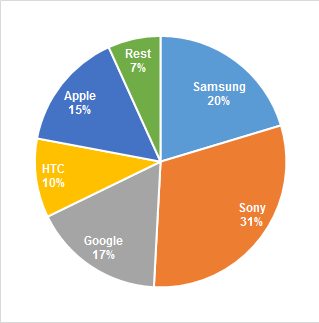
\includegraphics[scale=.4]{img/measure2-brands}
	\caption{Diversity of device brand sampled in measurements II}
	\label{fig:brandII}
\end{figure}

\subsection{Permanence of accelerometer}
When choosing biometric trait one of the factors is permanence described in \sectionref{auth:bio:character}, that is the trait not changing significantly over time. To test this measurement II were performed on a \textit{Sony Xperia Z1 Compact} over a period of 50 days. The choice of device was based on that \textit{Sony Xperia} devices is 30\% of the devices that data is collected from. The same test were also made on a \textit{Google Nexus 7} tablet. The graphs below shows the difference of accelerometer readings over time.
\begin{figure}[H]
	\centering
	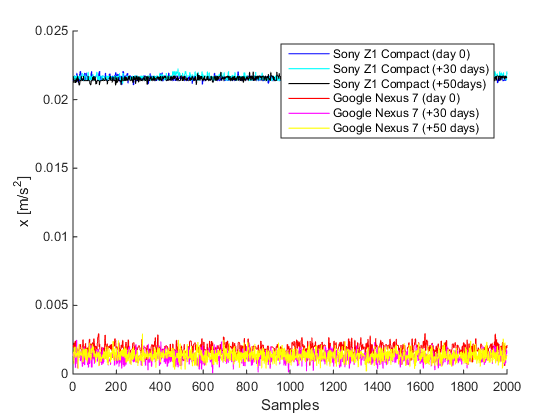
\includegraphics[scale=.7]{img/sensrec-nex-z1-acc-x}
	\caption{Accelerometer readings of x-axes on a  \textit{Sony Xperia Z1 Compact} and a \textit{Google Nexus 7} over 50 days}
	\label{fig:x50days}
\end{figure}
\begin{figure}[H]
	\centering
	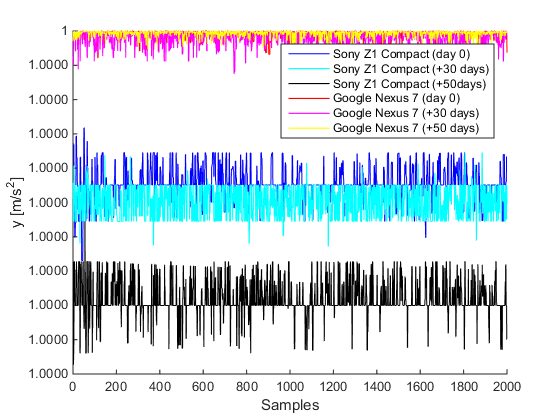
\includegraphics[scale=.7]{img/sensrec-nex-z1-acc-y}
	\caption{Accelerometer readings of y-axes on a  \textit{Sony Xperia Z1 Compact} and a \textit{Google Nexus 7} over 50 days}
	\label{fig:y50days}
\end{figure}
\begin{figure}[H]
	\centering
	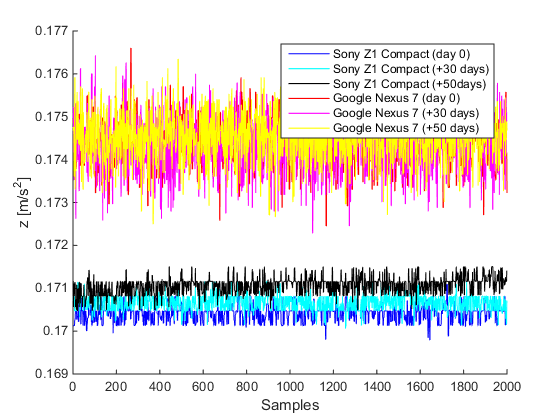
\includegraphics[scale=.7]{img/sensrec-nex-z1-acc-z}
	\caption{Accelerometer readings of z-axes on a  \textit{Sony Xperia Z1 Compact} and a \textit{Google Nexus 7} over 50 days}
	\label{fig:z50days}
\end{figure}
As seen in the figures the \textit{Google Nexus 7} hasn't changed much over the 50 days compared to the \textit{Sony Xperia Z1 Compact} that especially has changed in the y-axis. The reason for the difference of accelerometer change over time may be due to the \textit{Google Nexus 7} has only been in the same place during those 50 days and only used when the tests performed. Unlike Mobile used daily, may be dropped at some time. An additional fact about the measurements is that both devices has changed its OS between measurements 2 and 3. The \textit{Google Nexus 7} from Android KitKat 4.4.4 to Lollipop 5.1.1 and the \textit{Sony Xperia Z1 Compact} from Android KitKat 4.4.4 to CyanogenMod 12.1 ( Android version 5.1.1). \\
To get an perspective on this measurements among more devices the scatter-plot in~\figureref{fig:scatterSony50days} that include the same measurements from \textit{Sony Xperia Z1 Compact} as in~\figureref{fig:x50days},~\figureref{fig:y50days} and~\figureref{fig:z50days}.
\begin{figure}[H]
	\centering
	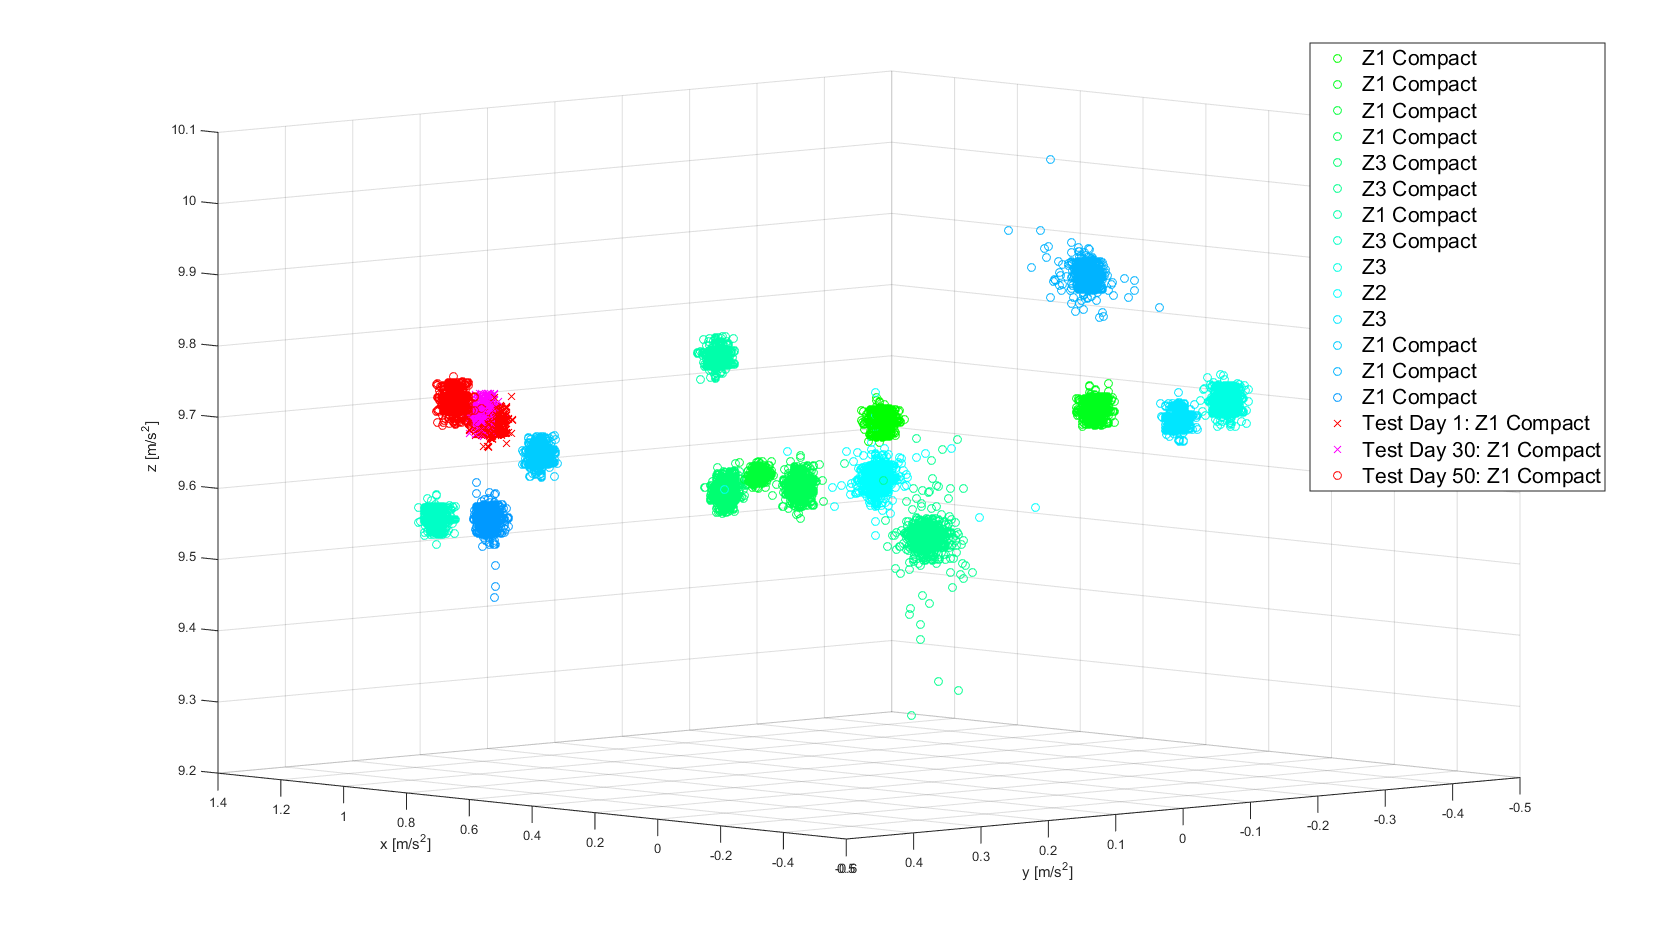
\includegraphics[scale=.3]{img/senrec-sony_scatter-2}
	\caption{Scatter-plot of accelerometer readings \textit{Sony Xperia}-device, one of them with measurements performed on the same device with 50 days apart.}
	\label{fig:scatterSony50days}
\end{figure} 

\subsection{Features of accelerometer data}\label{sec:featuresAcc}
As in ~\cite{sensor:accelPrint} I used statistical features calculated by the time domain. The features used and calculated as followed:
% === IfTime Gör en egen tabell!!
\begin{figure}[H]
	\centering
	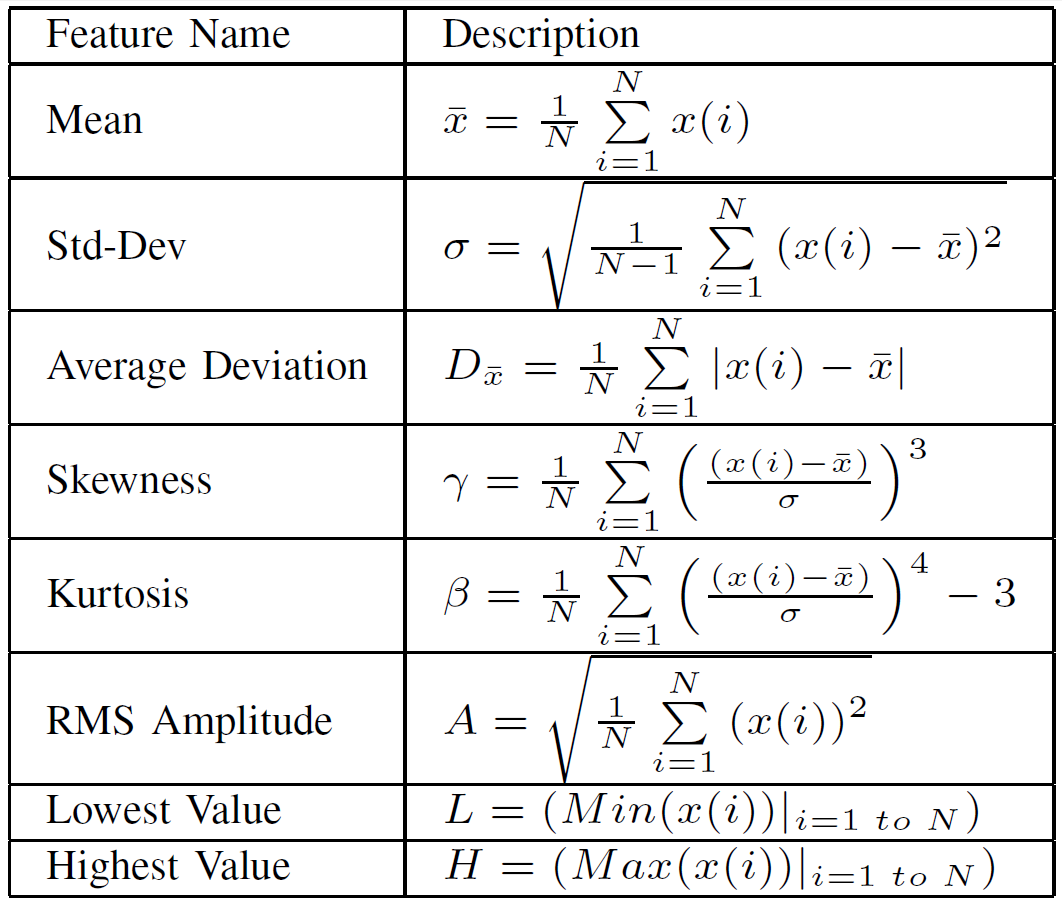
\includegraphics[scale=.35]{img/featureCalc}
	\caption{Calculations of statistical accelerometer features. \\\textit{From~\cite[p.6]{sensor:accelPrint}}}
	\label{fig:accFeatures}
\end{figure}
To compare these features and get a picture of if any of them are good for fingerprinting plots of devices were made. These can be found in~\appendixref{cha:matlabFeaturesPlot}. The chosen devices for the plots is the twelve \textit{Sony Xperia Z}-devices including the \textit{Sony Xperia Z1 Compact} that have measurements over 50 days. It becomes clear in the plots that almost all av the features is not changing over time. The only values that changing is the RMS and that the value would change was known even before because as seen in figure~\ref{fig:scatterSony50days} samples is changing over time, which is directly linked to the RMS.

% ToDo Tabell med värderna från min mobil tillsammans 
% med ngn form av snittdistans mellan punkterna om det går
% Lägga till nexus också!!
\begin{table}[H]
\begin{tabular}{| p{1cm} | p{1cm} | p{2.5cm} | p{1.8cm} | p{3.5cm} |} 
	\hline
  Feature 	& Day 0 & Day 30 & Day 50 & Median dist. 	\\ \hline
  Mean 		& 0 	& 		& 		& \%		\\ \hline
  Std. dev. & 0 	& 30 	& 50 	& \%	\\ \hline
  Avg. dev 	& 0 	& 30 	& 50 	& \%	\\ \hline
  Skewness 	& 0 	& 30 	& 50 	& \%	\\ \hline
  Kurtosis 	& 0 	& 30 	& 50 	& \%	\\ \hline
  RMS 		& 0 	& 30 	& 50 	& \%	\\ \hline
  Min 		& 0 	& 30 	& 50 	& \%	\\ \hline
  Max 		& 0 	& 30 	& 50 	& \%	\\ \hline
\end{tabular} 
\caption[Table caption text]{Values of features of \textit{Sony Xperia Z1 Compact} over 50 days together with the median distance between points of all measured devices.} \label{table:feature50}
\end{table}

\subsection{Gyroscope}
Lägg till ngn plot och visa hr ostabilt gyroskopet är mellan

\subsection{Simulate authentication of motion sensors in MATLAB}
To test that the features above is way of fingerprinting devices a simulation were performed in MATLAB. The concept is that a fingerprint of all devices is calculated. It contains all the features described in~\section{sec:featuresAcc}. When a new measurement is sent in to the simulation, features are calculated and compared to the once already known devices. The comparing is done by an algorithm that calculates the minimum distance between the features of the input device and the one already known. The distance is then used to decide if there is a match or not. As in biometric system there is a reashhold that decides how far from the values an input can be and sill be a match. This treashhold creates a rate of match error in the system called FRR and FAR (see~\sectionref{sec:bio:measure}). 
%% FAR FRR dör tabell eller ngt

% ========== CAMERA TEST ==========
\section{\textbf{ToUpdate! }Result Camera-measurements}\label{sec:ResCam}
\textbf{ ==== OBS!! ====}\\ Flyttad text som måste skrivas om.\\
\\
For the test of the camera sensor the PRNU value is calculated as an approximation of the algorithm described in section ~\ref{sec:char:camera} and also used by \cite{sensor:camera:DCIdent}. That is the average of multiple pictures used and substantially an approximation of \textit{f}. The first step is to remove the pictures-content which leaves the noise, which is done using a denoising filter. For the test the MATLAB \texttt{medfilt2} is used, which is an 2-D median filtering that outputs the median value of each pixel by its 3-by-3 neighbors. 
\begin{figure}[H]
  \centering
  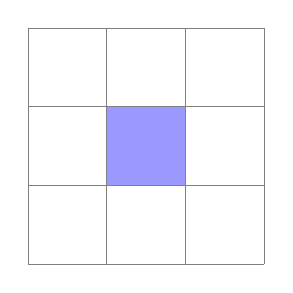
\begin{tikzpicture}[scale=1]
	\draw[step=1cm,gray,very thin] (0,0) grid (3,3);
	\fill[blue!40!white] (1,1) rectangle (2,2);
\end{tikzpicture}
  \caption{\label{fig:medfilt2} the MATLAB \texttt{medfilt2} outputs the median of each pixel by it's 3-by-3 neighbors}
\end{figure}
From the \texttt{medfilt2} we gain a picture without noise which is then subtracted from the original to get the noise. This technique works best if there are no features on the pictures such auto-fix, black and white etc. The more images used for the average value the better noise is, thus the amount random noise is less and the fixed noise is more. \cite{sensor:camera:DCIdent} recommend a minimum of 50 images. This is then seen as the reference pattern used for correlating the noise from another pictures. This correlation is calculated like:
$$
corr(\boldsymbol{n},\boldsymbol{r}) = 
\frac{(\boldsymbol{n} - \bar{\boldsymbol{n}})(\boldsymbol{r} - \bar{\boldsymbol{r}})}
{\|\boldsymbol{n} - \bar{\boldsymbol{n}}\| \|\boldsymbol{r} - \bar{\boldsymbol{r}}\|}
$$
A threshold for acceptance on correlation is found by experimental on images taken with or without the camera. Then there is a balance between FAR and FRR. 
In section ~\ref{sec:measurement:camera} i described two test preformed on the camera sensor of mobile devices.
\subsection{\textbf{ToDo! }Result of camera measurement I}
Since the purpose of this thesis compared to earlier work REFERENSER!! has the purpose of authentication and not forensics, is convenience for the collecting and measurability a factor to take in account. That is why the fist experiment is asked the users to record a 5 seconds video-clip with the device camera facing down on a flat object, like a table. Instead of making the user take 50 pictures or more which takes a lot of more time. This also makes it easier to get better noise since the same scene is used every time. \\
The video is then shuttled into images (100-200 from a 5 seconds video depending on fps on recording camera) that is used for calculating the PRNU. The MATLAB code for this is:\\
\rule{\textwidth}{0.5pt}
  \lstinputlisting{code/video2prnu1.m}
\rule{\textwidth}{0.5pt}

To compare an pictures between all collected PRNU the same calculation to get the noise is done. Then the noise from the reference pictures is compared to all collected PRNU and correlation is calculated like the formula above in MATLAB:\\
\rule{\textwidth}{0.5pt}
  \lstinputlisting{code/corrCamTest1.m}
\rule{\textwidth}{0.5pt}

\subsection{\textbf{ToDo! }Result of camera measurement II}
Since the earlier test leaved out some of the PRNU noise when recorded a video instead of taking a picture the new test consist of 10 images from every device. The recommendation from \cite{sensor:camera:DCIdent} to use at least 50 images is here compensated by again using black images (picture taking with device camera facing down). Since the scene is always the same the noise removal will be better in fewer images. The same code is used as above with the different that the video to image step is removed. The sizes of the images in this case is better since the camera on the mobile devices by default uses higher resolution when taking a picture then when recording. 


\chapter{CONCLUSIONS}\label{cha:conculsions}
\section{Conclusions}\label{sec:conculsions}
TODO!
\section{Ethical aspects}\label{sec:ethical}
TODO!
\section{Further work}\label{sec:further}
TODO!

\part*{Appendix}
\appendix
\chapter{Trista saker}\label{cha:boring}
Långa beräkningar brukar bli rätt trista\dots

Detta är ett appendix-kapitel.  Jämför med appendixet i \chapterref{cha:result}.

\section{Bädda sängen}

Den här beräkingen är så trista att vi kallar den \emph{att bädda sängen}.

\section{Diska}

Den här beräkingen är så trista att vi kallar den \emph{att diska}.

%\chapter{\rtthesis documentation and \LaTeX{} tips}\label{cha:rtthesis}

This document is not only an example that you can use to get started with the \rtthesis class, it also contains written instructions for how to use the class, and some general tips on how to use \LaTeX{} to produce a beautiful thesis.  As we do so in this chapter, we also get the opportunity to look at some theorem-like environments, which you can alter the look of by changing the options given to the \rtthesis class.

\section{Basic setup}\label{sec:basic-setup}
%
You must decide on an input encoding from start, and select the corresponding class option from \tableref{tab:inputenc} on \pagepageref{tab:inputenc}.  You must also tell \rtthesis whether you intend to use part sectioning or not, see \tableref{tab:part-options}.  There are many more class options, but they will be mentioned below where there is room for a more detailed discussion for the corresponding features.

Information about the thesis, which is needed to produce the thesis itself as well as the thesis cover and the “spikblad”, is passed to \rtthesis using the command \texcommand{setupThesis}.  The command is called in the following way, where the most common key-value pairs are listed in \tableref{tab:setupThesis} (the remaining key-value pairs concern master's theses, see \sectionref{sec:msc})):

\begin{minipage}{1.0\linewidth}
  \verbatimsize
\begin{verbatim}
\setupThesis{
  key1=value1,
  key2=value2,
  ...
}
\end{verbatim}
\end{minipage}

If a PhD thesis has an interesting illustration on the cover, it is customary to provide a caption for the illustration.  The caption will be printed on the back of the title page, and is set up by redefining the command \texcommand{rtcoverinfo}.  For instance, it may look like this:

\begin{minipage}{1.0\linewidth}
  \verbatimsize
\begin{verbatim}
\renewcommand{\rtcoverinfo}{\textbf{Cover illustration:}  Block
diagram showing the structure of the control scheme proposed in
\chapterref{cha:cool-control}}
\end{verbatim}
\end{minipage}


\begin{table}[tbp]
  \centering
  \caption{\label{tab:part-options}%
    Class options that inform \rtthesis whether part sectioning will be used or not.}

  \begin{tabular}{l p{0.5\linewidth}}
    \toprule%
    \textbf{Class option} & \textbf{Meaning} \\
    \otoprule%
    \classoption{parts} & Prepare for \texcommand{part} as the topmost sectioning command.\\
    \classoption{noparts} & Prepare for \texcommand{chapter} as the topmost sectioning command.\\
    \bottomrule%
  \end{tabular}
\end{table}

\begin{table}[tbp]
  \centering
  \caption{\label{tab:setupThesis}%
    Key-value pairs recognized by \texcommand{setupThesis}.  Note that values that include white space are surrounded by braces.}

  \begin{tabular}{>{\ttfamily}r !{\texttt{=}} >{\ttfamily}l p{0.5\linewidth}}
    \toprule%
    \textbf{Key} & \textbf{Example value} & \textbf{Comment} \\
    \otoprule%
    author & \{My Name\} & \\
    title & \{Thesis title\} & \\
    subtitle & \{Good stuff\} & Optional. \\
    city & Norrköping & Default: \emph{Linköping} \\
    year & 2010 & \\
    isbn & isbn-isbn-isbn-isbn & \\
    type & phd & Must be either \emph{phd}, \emph{lic}, or \emph{msc}. \\
    thesisNo & 9999 & Number in series (the series is determined by the choice of thesis type). \\
    localID & 11 & Only used for licentiate's theses.  It is the last part of the local identifier \emph{\mbox{LIU-TEK-LIC-2010:11}} in this case.\\
    username & isyusername & Used to generate the author's email address. \\
    dedication & \{To my parents!\} & \\
    \bottomrule%
  \end{tabular}
\end{table}

\section{Page layout and related options}\label{sec:page-layout}
%
Theses are restricted to the S5 paper size.  How the S5 page is organized is up to you, but \rtthesis only allows you to choose from two predefined layouts, and only one of them is recommended.  To get your own layout you should make a copy of \textfilename{rtthesis.cls} and modify the code for one of the existing class options for layout.  The class options for page layout are given in \tableref{tab:page-layout}.

At the time of writing, the printers used by LiU-Tryck print on A4 paper (physical size), which is then cropped to S5 (logical size).  Similarly, when you print draft versions of your thesis on your office printer, it is very likely that the used physical paper size will be A4.  Hence, it makes sense to let \rtthesis control how the S5 logical page is placed on the A4 physical paper.  In this case, \rtthesis will produce a \textsc{pdf} with pages in the A4 format, with content restricted to the S5 format.  On the other hand, when you produce a \textsc{pdf} that is meant to be read on a computer screen, the page size should be exactly S5.  When targeting the A4 physical format, it is possible to get crop marks for the S5 box, and to put some information about each page outside the S5 box.  The related class options are given in \tableref{tab:page-layout}.

To ensure that you really get the page layout you think when you send your thesis file to the printer's, the best option \emph{should} be to use the \classoption{crop} option.  However, they will tell you differently, since they think it's \emph{their} job to position the logical page on A4 and add crop marks.  Unfortunately, there is a lot of manual work in the process, so there is a (substantial?!) risk that the content of your pages will be shifted with respect to the S5 box of your layout\ldots

\begin{table}[tbp]
  \centering
  \caption{\label{tab:page-layout}%
    Class options related to page layout.  The most important one to remember is \classoption{crop} (since  \classoption{S5} and \classoption{pdf} are default).}

  \begin{tabular}{l p{0.5\linewidth}}
    \toprule%
    \textbf{Class option} & \textbf{Meaning} \\
    \otoprule%
    \classoption{S5} & Recommended layout.  Margin paragraphs are tiny (see \sectionref{sec:research:history} for examples), and should only be used for comments that will be removed in the final version of the thesis.  Default.\\
    \classoption{S5MP} & Layout to use if you are serious about margin paragraphs.  Not recommended, since the S5 format is too narrow to really fit margin paragraphs of reasonable width. \\
    \classoption{nailing} & Layout for the “spikblad”.  Not for theses! \\
    \midrule%
    \classoption{pdf} & Produce pages in the S5 format.  Default.\\
    \classoption{onA4} & Logical S5 page on a \textsc{pdf} page of size A4.\\
    \classoption{info} & Write information about each page above the logical S5 page.\\
    \classoption{crop} & Same as \classoption{onA4} with \classoption{info} and crop marks.\\
    \classoption{noInfo} & Turn off the effect of \classoption{info}.\\
    \classoption{draft} & Same as \classoption{onA4}, but pictures are blank and overfull \texttt{hbox}es stand out.\\
    \bottomrule%
  \end{tabular}
\end{table}

Although only weakly related to page layout, this section ends with a tip for how to change the size of the chapter numbers (some users find them much too big).  The font is controlled using the \styname{sectsty} package, and it follows that it can be redefined by, for instance,

\begin{minipage}{1.0\linewidth}
  \verbatimsize
\begin{verbatim}
\chapternumberfont{\fontsize{60mm}{63mm}\selectfont}
\end{verbatim}
\end{minipage}

\section{Front-matter environments}

There are environments defined for typical sections in the front-matter\footnote{The \emph{front-matter} is everything that goes in the beginning of the thesis, before the page numbered~\emph{1}.}.  The most important purpose of providing these environments is that they take care of the table of contents and the \textsc{pdf} bookmarks for you.  The environments are \envname{abstract}, \envname{preface}, \envname{acknowledgments}, and \envname{notation}.

The environment \envname{abstract} accepts the language used inside the environment as an optional argument (which defaults to \texttt{english}).  If the language is set to \texttt{swedish}, the title of the abstract will be \emph{Populärvetenskaplig sammanfattning}, in accordance with the Linköping University requirements on theses written in English.

Inside the \envname{notation} environment, you can put anything you like, and maybe the \envname{notationtabular} environment provided by \rtthesis suits your needs.  In order to define this environment, \rtthesis loads the two packages \styname{array} and \styname{ctable}, and also defines the command \texcommand{otoprule} to mean the same as \texcommand{toprule}.  See \tableref{tab:notationtabular} regarding how to change the look of \envname{notationtabular}.

\begin{table}[tbp]
  \centering
  \caption{\label{tab:notationtabular}%
    Legal option values to the \envname{notation} environment.  The options control the look of the \envname{notationtabular} environments used inside the \envname{notation} environment.  The initial definition of \envname{notationtabular} is the same as that obtained by passing the option \classoption{new}.}

  \begin{tabular}{l p{0.5\linewidth}}
    \toprule%
    \textbf{Option} & \textbf{Meaning} \\
    \otoprule%
    \emph{emty} & Do not redefine \envname{notationtabular}.  Default.\\
    \classoption{old} & Make \envname{notationtabular} produce a plain \LaTeX{} table with double horizontal lines under the table headings, and a vertical line separating the two columns.\\
    \classoption{new} & Make \envname{notationtabular} produce a table according to the guidelines in \citet{Mori07Tables} using the \styname{ctable} package.\\
    \bottomrule%
  \end{tabular}
\end{table}

There is a class option called \classoption{noextras}, which was intended to inhibit the effect of the \texcommand{maketitle} command, and redefine the front-matter environments to not produce any output.  However, the option is not working well at the moment.  On the other hand, as the time it takes to compile a thesis on a modern computer is very short, it is rather unclear why someone would like to use this feature anyway.


\section{Abbreviations}

Automatic control is a \LaTeX{}-friendly community.  This means that everything you produce is expected to look good.  We begin with a basic result.

\begin{theorem}\label{th:abbr-in-sc}
  Abbreviations, such as \abbrARMA, look best in small caps.

  \begin{proof}
    Just compare with “ARMA”.
  \end{proof}
\end{theorem}

However, it is important that the small caps match the sorrounding text, compare the statement in the theorem above with the following variation of it, in italics instead of slanted text:
\begin{quotation}
  \noindent\textit{Abbreviations, such as \abbrARMA\footnote{This will cause a \LaTeX{} warning.} or {\normalfont\textsc{arma}}, will stick out in a terrible way if you don't watch out!}
\end{quotation}
This is why the \rtthesis class uses slanted text rather than italics in theorems rather when slanted small caps are available.

Unfortunately, \rtthesis does currently not provide a way to make small caps look good in italics, which leads to the following corollary to \theoremref{th:abbr-in-sc}.

\begin{corollary}
  One has to make a choice between
  \begin{itemize}
  \item Beautiful abbreviations using small caps (instead of ordinary upper case).
  \item Pretty text typeset in italics (instead of slanted text).
  \end{itemize}
\end{corollary}

\section{Definitions}

Let us discuss another theorem-like environment while we have some examples of similar environments to compare with in the previous section.  That is, let us discuss the \envname{definition} environment (and the similar environments \envname{assumption} and \envname{remark}).  All the theorem-like environments are defined in a separate package, \styname{rtthesis-theorems}, so that they can be used with other document classes as well.  The definition below is an example of a definition with a title.

\begin{definition}[Definition]
  A \emph{definition} is a precise explanation of the meaning of a word or concept.  It may be tempting to include examples in a definition, but a good definition should not depend on examples as part of the definition.  However, examples are often useful to clarify a definition, and should appear near the definition.

  A short definition may require just a single paragraph, while a more complex definition may require a few paragraphs.  Some definitions will also make use of displayed math.
\end{definition}

One problem one has to consider if definitions are not restricted to just one paragraph, is how to show the reader where the definition ends.  In theorems, it is common to use italics or slanted text (for brevity, we will not mention italics from here on) to show where the theorem statement ends, but for definitions it may be desirable to use the slanted text to emphasize the word or concept being defined.  (It is arguably more clear to highlight the new word or concept using slanted text with upright surrounding text, than vice versa.)  To use an upright font for the definitions may also be a way of avoiding to heavy use of slanted text.

Various options related to the appearance of theorem-like things (in \LaTeX{}, a definition is a kind of theorem) are described in \tableref{tab:theorems}.  \Tableref{tab:definitions} (used also to illustrate tables) contains some suggestions regarding combinations of options for the \envname{definition} environment and options for paragraph breaks.

\begin{table}[tbp]
  \centering
  \caption{\label{tab:theorems}%
    Class options related appearance of theorem-like environments.  The \emph{theorem-like environments} defined by \rtthesis are \envname{theorem}, \envname{proposition}, \envname{lemma}, \envname{corollary}, \envname{definition}, \envname{assumption}, and \envname{remark}.  The \emph{definition-like environments} are a subset of the \emph{theorem-like environments}, consisting of the environments \envname{definition}, \envname{assumption}, and \envname{remark}. See also \tableref{tab:fonts} regarding the fonts used in theorems.}

  \begin{tabular}{l p{0.5\linewidth}}
    \toprule%
    \textbf{Class option} & \textbf{Meaning} \\
    \otoprule%
    \classoption{break} & Put line breaks after the titles of the environments \envname{theorem}, \envname{proposition}, \envname{lemma}, and \envname{corollary}.\\
    \classoption{nobreak} & Never put line breaks after titles of theorem-like environments.  Default.\\
    \midrule%
    \classoption{definition=naked} & Definition-like environments look like the surrounding text, and are only isolated by some vertical white space.  Default.\\
    \classoption{definition=theorem} & Definition-like environments use same font as the \envname{theorem} environment, and are isolated by some vertical white space.\\
    \classoption{definition=marks} & Definition-like environments look like the surrounding text, and are isolated by small marks.  Strongly recommended if \classoption{parskip} is used.\\
    \midrule%
    \classoption{nosharecounter} & Use separate numbering sequences for each theorem-like environment and the \envname{example} environment.\\
    \classoption{sharecounter} & Use one numbering sequence for theorem-like environments, and the \envname{example} environment.\\
    \bottomrule%
  \end{tabular}
\end{table}

Sometimes, a definition may be given without a title.  The next definition is an example of this, even though it is questionable whether it was a good idea to omit the title in this particular case.

\begin{definition}
  An \emph{environment} in \LaTeX{} is a construct that is entered with the command \texcommand{begin\{\ldots\}} and exited with the command \texcommand{end\{\ldots\}}, where “\ldots” should be the name of the environment.
\end{definition}

In \tableref{tab:theorems}, there are three options related particularly to how \envname{definition}, \envname{assumption}, and \envname{remark} are typeset.
\begin{itemize}
\item With \classoption{definition=naked} (default) the definitions are typeset in upright font, and there is nothing on the page that marks the end of the definition.
\item With \classoption{definition=theorem} the definitions are typeset in the same style as theorems.  Since theorems are supposed to be typeset in slanted text, this will make it clear where the definition ends.
\item With \classoption{definition=marks} the beginning and end of definitions will be indicated with small marks.  Compare how the end of a proof is marked with a square box!  The current implementation has some problems with placing the marks if the definition ends with a displayed equation, but this can be compensated for by manual insertion of a \texcommand{vspace} command.
\end{itemize}

You may judge from the following example whether manual insertion of a \texcommand{vspace} command is necessary to make the definition ending with a displayed equation look alright.

\begin{definition}
  The factorial (denoted by the postfix operator $!$), defined for natural numbers, is given by
  \begin{equation*}
    n! =
    \begin{cases}
      1, & \text{if $n = 0$} \\
      n \cdot (n-1) \cdot \dotsc \cdot 1, & \text{otherwise}
    \end{cases}
  \end{equation*}
\end{definition}

This paragraph only serves to highlight the vertical white space below the definition ending with a displayed equation.  Note that one way to avoid problems with this kind of definitions is to rewrite them so that they don't end with displayed equations.

All definitions in this section have been entered as isolated paragraphs; that is, there is an empty line in the source code of the document before and after each \envname{definition} environment.  Although not recommended, \rtthesis supports definitions that are connected with the preceding paragraph, in which case the usual vertical space (if any) between paragraphs will not be inserted.  \emph{Be careful so that you don't omit the paragraph breaks by mistakes, since it makes a difference that may be hard for proofreaders to spot!}  As an example of a definition written in the same paragraph as the preceding text,
\begin{definition}
  A \emph{paragraph} (according to Oxford American Dictionaries) is a distinct section of a piece of writing, usually dealing with a single theme and indicated by a new line, indentation, or numbering.
\end{definition}
There is no paragraph break in the source code between the definition above and this text, but currently this cannot be seen in the typeset document.  If you know how to solve this, let the \rtthesis maintainer know!  If you want to learn about the \TeX{} mechanisms involved, see \citet{RyckoJackowski93TeXIndentPar}.

\section{Theorem titles}
%
The class lets you control the white space that separates a theorem title from the theorem statement.  The options appear in \tableref{tab:theorems}.  With the class option \classoption{break} (default), you will get a line break.  With \classoption{nobreak}, you will just get horizontal space.  Not all types of theorem-like environments will be affected by the \classoption{break} option, so to get things exactly they way you want, you may have to make your own modified copy of the \rtthesis class.  Try to recompile the document with the two different options and compare the result!

\section{To share or not to share counters}\label{sec:rtthesis:sharecounter}
%
Other things to think about regarding style include whether to use the same counter for all sorts of theorem-like things.  Again, the options appear in \tableref{tab:theorems}.  Some like to make the number of important theorems to stand out by having a separate counter (as in \citet{Khalil02NonlinearSystemsBook}), while other prefer to use as few counters as possible in order to make it easy to locate referenced items (as in \citet{Rugh96LinearSystemsBook}).  The two alternatives are supported in \rtthesis, via the options \classoption{sharecounter} and \classoption{nosharecounter}.

\section{Completely customized theorem-like environments}\label{sec:rtthesis:custom-theorems}
%
If you don't like the way \rtthesis sets up theorem-like environments (listed in the caption of \tableref{tab:theorems}) for you, you may pass the class option \classoption{notheorems}.  Then \styname{amsthm} will not be loaded, none of the theorem-like environments will be defined, and it is up to you to define your own environments.  If you decide to do so, using the \styname{amsthm} package will be a good idea.

\section{The \envname{example} environment}
%
The \envname{example} environment defined by the \rtthesis class is \emph{not} a floating environment, but is simply used to highlight that the text inside the environment is just an example of something more general that you have explained before.  Just as with the theorem-like environments, the environment is defined in a separate package, \styname{rtthesis-example}, so that it can be used with other document classes as well.

\begin{example}
  As an example of the \envname{example} environment, we include a little example here.  You can use this example to see how the options described in \sectionref{sec:rtthesis:sharecounter} affects the numbering of the environment.

  Depending on where this example ends up in the typeset document, you may also have the chance to see the ugly stretched vertical space that sometimes appears at the top and bottom of the environment.
\end{example}

There are three lengths you may play with the fine tune the appearance of examples, explained in \tableref{tab:example-lengths}.  Clearly, it would be possible to introduce additional parameters, but currently the corresponding aspects of the environment are hard-coded into \rtthesis.

\begin{table}[tb]
  \centering
  \caption{\label{tab:example-lengths}%
  The lengths used to control the appearance of the \envname{example} environment.  Note that the environment tries to compensate for the current value of \texcommand{parskip}, so you may not always get exactly what you'd expect.  Also, the meaning of the distance between the upper stroke and the text is somewhat arbitrary in order to allocate space for the example title.}

  \begin{tabular}{>{\small\ttfamily}l p{0.1\textwidth} p{0.4\textwidth}}
    \toprule
    {\normalsize\normalfont\textbf{Length}} & \textbf{Default} & \textbf{Purpose} \\
    \otoprule
    $\backslash$exampleLineWidth & $\unit{0.6}{pt}$ & Thickness of the strokes. \\
    \midrule
    $\backslash$exampleTopBotInnerMargin & $\unit{2}{ex}$ & Vertical space between strokes and contents of the example. \\
    \midrule
    $\backslash$exampleTopBotOuterMargin & $\unit{1}{em}$ \texttt{plus} $\unit{1}{ex}$ \texttt{minus} $\unit{1}{ex}$ & Vertical space surrounding the example. \\
    \bottomrule
  \end{tabular}
\end{table}

As is mentioned in the example above, there is sometimes problem with vertical space at the top and bottom of the \envname{example} environment.  During the page breaking process (see \sectionref{sec:tipt:page-breaking}) you could consider to add something like
{\verbatimsize
\begin{verbatim}
  \vspace{-1\baselineskip}
\end{verbatim}}
to reduce such artifacts.  Even better, if you know how to correct this in the definition of the environment, let the \rtthesis maintainer know!  The paper \citet{RyckoJackowski93TeXIndentPar} is recommended for anyone interested in the lesser known details of \TeX{} that one has to grasp in order to really solve the problem.

\section{Captions}\label{sec:rtthesis:captions}
%
The \rtthesis class loads the \styname{captions} package to obtain good-looking captions.  Captions are set up assuming that table captions will be placed above the table they belong to.  Many authors find this confusing since figure captions are always placed below the figure they belong to.  If you want to put table captions below the table you need to adjust the spacing around the caption by putting the following line in your personal style file:
{\verbatimsize
\begin{verbatim}
\captionsetup[table]{position=bottom}
\end{verbatim}}

Note that the command above only changes the spacing around the caption.  You still have to put the code for each caption relative to the tabular itself consistently with the captions setup.  Two tables are included in this document for illustration.  \Tableref{tab:definitions} indicates the many combinations of options that the \envname{definition} environment has been designed to work with.  The next one, \tableref{tab:chapters} is just a stupid table telling where the different chapters in this document begin.  For comparison, a typical automatic control block diagram has been included in \figureref{fig:feedback}.

Some nice guidelines for table creation in \LaTeX{} are given in \citet{Mori07Tables} (it is just two clicks away!).

\begin{table}[p]
  \centering
  \caption{\label{tab:chapters}%
    Different combinations of class options that affects the \envname{definition} environment.  The code for this caption appears at the beginning of the \envname{table} environment.  It would have had the desired distance to the tabular if the default caption setup of \rtthesis was used, but this document has been set up for table captions below the corresponding tabular.}
  \begin{tabular}{c l c}
    \toprule%
    \textbf{Chapter} & \textbf{Title} & \textbf{Page} \\
    \otoprule%
    \ref*{cha:intro} & \nameref{cha:intro} & \pageref{cha:intro} \\
    \ref*{cha:Research} & \nameref{cha:Research} & \pageref{cha:Research} \\
    \ref*{cha:rtthesis} & \nameref{cha:rtthesis} & \pageref{cha:rtthesis} \\
    \ref*{cha:boring} & \nameref{cha:boring} & \pageref{cha:boring} \\
    \bottomrule%
  \end{tabular}
\end{table}

\begin{table}[p]
  \centering
  \caption{\label{tab:definitions}%
    Different combinations of class options that affects the \envname{definition} environment.  The code for this caption appears at the end of the \envname{table} environment.  It will be too close to the tabular using the default settings of \rtthesis (but note that this document has been setup differently, see \sectionref{sec:rtthesis:captions}).}

  \begin{tabular}{>{\bfseries}l c c c}
    \toprule%
    & \multicolumn{3}{c}{\bfseries\texttt{definition=}} \\
    & \bfseries\classoption{naked} & \bfseries\classoption{theorem} & \bfseries\classoption{marks} \\
    \otoprule%
    \classoption{noparskip} & OK & Avoid & OK \\
    \midrule
    \classoption{parskip} & Bad & Avoid & OK \\
    \bottomrule%
  \end{tabular}
\end{table}

\begin{figure}[p]
  \centering
  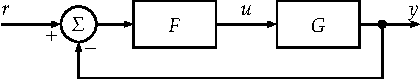
\includegraphics{feedback}
  \caption{\label{fig:feedback}%
    A simple illustration in a floating \envname{figure} environment.  Note that figure captions are always placed under the corresponding figure, and hence that the caption code should always appear at the end of the \envname{figure} environment.}
\end{figure}

\section{Hyperlinks}
%
For readers our the electronically published version of your thesis, as well as yourself while your are working on it, it is very convenient to have working hyperlinks in the document.

\subsection{Basic setup}
%
Basically, hyperlinks are obtained by using the \styname{hypreref} package. However, this package has quite a lot of compatibility issues with other packages, and knowledge about how to deal with these issues is coded into the \rtthesis class.  That is, all you should have to do to get hyperlinks in your document is to specify the \classoption{hyperref} option to \rtthesis.  The class options related to the linking infrastructure of the document are listed in \tableref{tab:hyperref}.

At the time of writing \rtthesis does not call \texcommand{hypersetup} with information about document title, keywords, and other information provided to \texcommand{setupThesis} (see \tableref{tab:setupThesis}).  If someone wants this, it shouldn't be hard to do.

\begin{table}[tbp]
  \centering
  \caption{\label{tab:hyperref}%
    Class options related to (hyper) linking infrastructure.}

  \begin{tabular}{l p{0.5\linewidth}}
    \toprule%
    \textbf{Class option} & \textbf{Meaning} \\
    \otoprule%
    \classoption{hyperref} & Turn on hyperlinks using the \styname{hyperref} package.  Default. \\
    \classoption{nohyperref} & Turn off hyperlinks, and compensate for commands no longer provided by the \styname{hyperref} package. \\
    \midrule%
    \classoption{backref} & Turn on bibliography back references.  Default. \\
    \classoption{nobackref} & Turn off bibliography back references.  (Currently required if you plan to use the features of \styname{bibunits}.)\\
    \bottomrule%
  \end{tabular}
\end{table}


\subsection{Hyperlinks and electronic publishing}
%
To make your dear hyperlinks survive all the way to the electronic publishing system, you may have to replace the file that is sent to e-press by LiU-tryck.  The problem is that LiU-tryck creates a compressed version of the file that is used in the printer, and the compression will remove nice features such as page numbers, hyperlinks, and bookmarks.  Fortunately, the guys at e-press seem to be understanding and will accept to publish a file that they receive directly from you.

\subsection{Page number formatting in the index}
%
If you use an index in your thesis, you will often want to change the formatting of certain page numbers in the index.  Without \styname{hyperref}, this could look like
{\verbatimsize
\begin{verbatim}
hyperlinks\index{hyperlinks|textit}
\end{verbatim}}
to get the page number for this occurrence of \emph{hyperlinks} to be typeset in italics.  The problem with this is that this page number will not be a hyperlink, while other page numbers will be hyperlinks to the correct page.  To get both italics and a hyperlink you need to define a special index formatting commands like the following.
{\verbatimsize
\begin{verbatim}
\newcommand{\hyperpageit}[1]{\textit{\hyperpage{#1}}}
\newcommand{\hyperpagebf}[1]{\textbf{\hyperpage{#1}}}
\newcommand{\hyperpagefootnote}[1]{\hyperpage{#1}n}
\end{verbatim}}

Now, you can write
{\verbatimsize
\begin{verbatim}
hyperlinks\index{hyperlinks|hyperpageit}
\end{verbatim}}
to get both italics and a hyperlink.  The \rtthesis class will provide a trivial definition of \texcommand{chapter} in case \styname{hyperref} is not loaded, so you may safely start to use the above definitions even if you are not sure whether you will use hyperlinks in the end.

\subsection{Friendlier hyperlinks}
%
The default mechanism for references in \LaTeX{}, being the command \texcommand{ref}, is modified as expected by the \styname{hyperref} package.  For instance, the number in “chapter~\ref{cha:rtthesis}” is linked to the beginning of the current chapter (if you click it, be sure to just the \emph{jump back} function of your \textsc{pdf} viewer to get back to here!).  However, all of “\hyperref[cha:rtthesis]{this}” is also a link to the same place.  That is, it is possible to other things than the number itself as links.  We could also make a reference that will never be linked, like in “chapter~\ref*{cha:rtthesis}”.

So, what's so friendly about this?  What I'm aiming at is that you can say “\hyperref[cha:rtthesis]{chapter~\ref*{cha:rtthesis}}”.  The code for this link is
{\verbatimsize
\begin{verbatim}
\hyperref[cha:rtthesis]{chapter~\ref*{cha:rtthesis}}
\end{verbatim}}

Of course, it is very annoying to repeat the key twice; first to point the hyperlink to the correct place, second to show the number of the chapter.  With the \texcommand{autoref} command from the \styname{hyperref} bundle, we get “\autoref{cha:rtthesis}”.  This is almost perfect.  The problem is that one cannot get an uppercase initial at the beginning of a sentence without redefining “chapter” to “Chapter“,
{\verbatimsize
\begin{verbatim}
\renewcommand{\Chaptername}{Chapter}
\end{verbatim}}
but then we will not get the nice lower case initial in the middle of a sentence.  Many authors don't bother about this and use uppercase initials irrespectively of where in a sentence the reference appears.

The only solution I (Henrik Tidefelt) knows of, is to define special commands for each type of reference.  A basic solution might look as follows.
{\verbatimsize
\begin{verbatim}
\newcommand{\chapterref}[1]{\hyperref[#1]{chapter~\ref*{#1}}}
\newcommand{\Chapterref}[1]{\hyperref[#1]{Chapter~\ref*{#1}}}
\end{verbatim}}

You should then use \texcommand{chapterref} in the middle of a sentence, and \texcommand{Chapterref} at the beginning of a sentence.  I you later decide that you want to have upper case initials everywhere, you just have to change your definitions to
{\verbatimsize
\begin{verbatim}
\newcommand{\chapterref}[1]{\hyperref[#1]{Chapter~\ref*{#1}}}
\newcommand{\Chapterref}[1]{\hyperref[#1]{Chapter~\ref*{#1}}}
\end{verbatim}}

A more complete solution will also provide commands for the plural forms “chapters” and “Chapters”.

It is also nice to use a similar technique for page references.  For instance, this chapter starts on \hyperref[cha:rtthesis]{page~\pageref*{cha:rtthesis}}, and such links can be created easily using a command like
{\verbatimsize
\begin{verbatim}
\newcommand{\pagepageref}[1]{\hyperref[#1]{page~\pageref*{#1}}}
\end{verbatim}}

Because of the many possible preferences for how to handle labels and references within documents, \rtthesis does not define any related commands.  The current section should give you some ideas of what can be achieved, and now it is up to you to design your own solution or borrow a solution from someone else (or simply stick with \texcommand{autoref} or the 1980's way of doing things)!

\section{Backreferences from the bibliography}
%
By default, \rtthesis uses the \styname{backref} package to put references from the bibliography back into the text.  The options for turning this feature on and off are listed in \tableref{tab:hyperref}.

By controlling this feature via the class, the choice whether to use it or not can be made orthogonal to the choice of whether to use \styname{hyperref} or not.

In addition to just loading \styname{backref}, \rtthesis will do a basic setup of the commands used to typeset the list of page numbers for each reference.  This behavior can easily be redefined without modifying the \rtthesis class file.  See the \styname{backref} documentation for details on how to do this!

\section{Using the \styname{bibentry} package}\label{sec:rtthesis:bibentry}
%
The \styname{bibentry} package makes it possible to use the information in the bibliography to present your publications at any place in the document.  In order to work independently of whether you use back references from the bibliography or not, you need to follow the pattern below each time you use the \texcommand{bibentry} command, where \texttt{KEY} is the same key to you publication that you would with use with any other citation command.

\begin{minipage}{1.0\linewidth}
  \verbatimsize
\begin{verbatim}
\begin{quotation}
  \nocite{KEY}\noindent
  \backrefparscanfalse\bibentry{KEY}.\backrefparscantrue
\end{quotation}
\end{verbatim}
\end{minipage}

To use the \envname{quotation} environment is just a suggestion — it will make the reference stand out by using a some what shorter text line width.  Note the period that follows the \texcommand{bibentry} command — the command leaves it up to you how to terminate the entry.  The \texcommand{nocite} command ensures that the reference appears in the bibliography, which is necessary to produce the entry.  The \texcommand{noindent} commands simply prevents the first line in the \envname{quotation} from being indented.  The commands \texcommand{backrefparscanfalse} and \texcommand{backrefparscantrue} are related to the \styname{backref} package used to produce back references from the bibliography, and should always surround the \texcommand{bibentry} command.  In case you have turned back references off using the \classoption{nobackref}, \rtthesis will provide substitutes for these two commands.


\section{Fonts}
%
Though basically not a task for a \LaTeX{} class, \rtthesis will assist in loading some font packages.  There are some class options that control this behavior, described below, and if these options are not good enough for you, you may have to make your own copy of the class and replace the font packages you don't like.  Options for font selection are listed in \tableref{tab:fonts}.

One reason, however, for letting \rtthesis handle the font selection is that this makes it possible for the class to do some things more intelligently.  At the moment, \rtthesis will help you make use of some of the goodies of KpFonts, if you choose to use that font.

\begin{table}[tbp]
  \centering
  \caption{\label{tab:fonts}%
    Class options related to fonts.  When slanted small caps are activated, theorem-like environments will use slanted text instead of italics.  The lower part of the table are examples of options that will be understood by the \styname{kpfonts} package, and are only meaningful in combination with the \classoption{kp} option.  (Note that options passed to \rtthesis, but that are not understood by \rtthesis will be passed on automatically by \LaTeX{} to loaded packages.)}

  \begin{tabular}{l p{0.5\linewidth}}
    \toprule%
    \textbf{Class option} & \textbf{Meaning} \\
    \otoprule%
    \classoption{kp} & Use KpFonts (Kepler) and activate slanted small caps.  Default.\\
    \classoption{times} & Use Times and deactivate slanted small caps.\\
    \classoption{lm} & Use Latin Modern and deactivate slanted small caps.\\
    \midrule%
    \classoption{largesmallcaps} & Let the small caps be slightly higher than an \emph{x}.  See the KpFonts documentation!\\
    \classoption{intlimits} & Placement of integration limits.  See the KpFonts documentation!\\
    \classoption{widermath} & Put just a little more horizontal space between entities in math mode.  See the KpFonts documentation!\\
    \bottomrule%
  \end{tabular}
\end{table}

\section{Hanging punctuation}
%
The \rtthesis class automatically loads the \styname{pdfcprot} package with its default settings.  It uses a pdf\TeX{} feature to make punctuation hang into the right margin.  If you don't like it, make your own copy of the class and comment out the line that loads the package.  One reason not to use it would be if your document will be (perhaps only occasionally) typeset using the old \TeX{} program, since this will lead to noticeable differences in the line breaks compared to when pdf\TeX{} is used.  No matter what you choose, make your choice \emph{before} you start working with the page breaks in your document!

\section{Paragraph breaks}
%
There are two common ways of visualizing paragraph breaks in a document, illustrated by the two examples below.  The look of paragraph breaks is controlled using the class options listed in \tableref{tab:parskip}.

\begin{table}[tbp]
  \centering
  \caption{\label{tab:parskip}%
    Class options related to formatting of paragraph breaks.}

  \begin{tabular}{l p{0.5\linewidth}}
    \toprule%
    \textbf{Class option} & \textbf{Meaning} \\
    \otoprule%
    \classoption{noparskip} & US style, see \exampleref{ex:paragraph-break-noparskip}.  Default.\\
    \classoption{parskip} & European style, see \exampleref{ex:paragraph-break-parskip}.\\
    \bottomrule%
  \end{tabular}
\end{table}

% \begin{example}[Default text]
%   This example does not mess with the lengths controlling the paragraph break format.  But you bet it ends in vmode!

% \end{example}

% It is good to see what it looks like if one puts text just below an example.

% \begin{example}[Default text]
%   This example does not mess with the lengths controlling the paragraph break format.  This one ends in hmode!
% \end{example}

\begin{example}[Indented first line]\label{ex:paragraph-break-noparskip}%
  \setlength{\parskip}{0pt}%
  \setlength{\parindent}{1.5em}%
  This style is still the most common.  It is particularly dominant in text written in the US.

  It is a matter of style whether to omit the indentation of the first line after a sectioning command such as \texcommand{chapter} or \texcommand{subsection}.  The omission is typically automated, but can also be enforced using the  \texcommand{noindent} command.

  One drawback of not having vertical space between paragraphs is that it will be harder for pdf\TeX{} to find good places for page breaks, compared to the option shown below.  If you like compact documents, however, this is the option for you!

  For testing purposes, this example ends with a paragraph break, so that \TeX{} is in \emph{vmode} at the end.  You should always avoid this, but the class will try to compensate for your mistakes\ldots

\end{example}

\begin{example}[Vertical white space]\label{ex:paragraph-break-parskip}%
  \setlength{\parskip}{1ex}%
  \setlength{\parindent}{0pt}%
  This style is still increasing in popularity.  It is rather common in modern texts written in Europe, and the style has received special attention from the Netherlands \TeX{} user group \emph{Nederlandstalige \TeX{} Gebruikersgroep, \textsc{ntg}}.  Their efforts can be used through their variants of the standard \LaTeX{} classes.

  Unfortunately, the \textsc{ntg} classes are not compatible with \rtthesis, and the solution provided by the \styname{parskip} package is only part of the solution.  Hence, \rtthesis will do more than just loading the \styname{parskip} package for you if you specify the \classoption{parskip} option.

  A good reason to put code related paragraph breaks in the class file is that all the small adjustments that different people come up with can be put in one placed so that they are accessible to future users of the class.
\end{example}

\section{Page breaks}\label{sec:tipt:page-breaking}
%
There is a whole lot to say about how to obtain nice page breaks.  You will find some recommendations below, but do not use this document as your ultimate reference on this topic!  (This document itself contains some really nasty page breaks --- at least at the time of writing this --- as a result of not paying any attention at all to the problem.  It would simply bee too time-consuming to keep adjusting the page breaks each time the document is edited.)
\begin{itemize}
\item
  Take no consideration of page breaks until page breaking is the only aspect of your thesis that remains to be taken care of!  Page breaking involves a lot of manual intervention of the automatic mechanisms in pdf\TeX{}, and as soon as you have started to intervene, any further changes to the text will risk to ruin your page breaking fixes, and may even lead to worse results than before since the automatic page breaking has been tampered with.
\item
  First thing to try is to make changes to the text to help the automatic page breaking mechanism.  Try to make sentences longer or shorter depending on the situation.  Since this will not tamper with the automatic page breaking mechanism, this option will incur the least loss of maintainability of your document.
\item
  Can the location of floats be changed to improve page breaks?  Play around with exactly where in your source files the code for the floating environments appears!
\item
  You may also try to force early page breaks using the \texcommand{Needspace*} command.  For instance, putting
{\verbatimsize
\begin{verbatim}
\Needspace*{2\baselineskip}
\end{verbatim}}
before a paragraph will cause a page break if there is not enough vertical space on the page to hold two lines of text.  The good thing about this option is that your intervention will cause no harm if the \texcommand{Needspace*} command appears in the middle of a page.  The bad thing about this option is that it may cause remaining vertical space on the broken page to be stretched quite badly.  You should always check that the resulting page looks OK!

For more information, and related commands, see the documentation for the \styname{needspace} package!
\item
  The last option is to play with the vertical size of individual pages.  For instance, putting
{\verbatimsize
\begin{verbatim}
\enlargethispage{2\baselineskip}
\end{verbatim}}
before a paragraph you would like to fit into the current page will make space for two extra lines of text.  This avoids the bad stretching of vertical space that the \texcommand{Needspace*} option may cause.  However, if you would make other changes that makes tampering with the page size unnecessary, it will be very time-consuming to detect this and remove the no longer needed \texcommand{enlargethispage} command.
\end{itemize}

Note that manual page breaking is a time-consuming task.  Make sure to have at least one full day allocated to page breaking before you submit your thesis for print!

\section{Input encoding}
%
Two input encodings are supported, being \mbox{latin-1} and \mbox{\textsc{utf}-8}.  The choice of input encoding should be made via the \rtthesis class, so that the class can use the correct encoding to define certain global strings.  The input encoding options are listed in \tableref{tab:inputenc}.

\begin{table}[tbp]
  \centering
  \caption{\label{tab:inputenc}%
    Class options related to input encodings.  Note that there is no default; \rtthesis requires one of these options to be passed explicitly.}

  \begin{tabular}{l p{0.5\linewidth}}
    \toprule%
    \textbf{Class option} & \textbf{Meaning} \\
    \otoprule%
    \classoption{latin1} & Simply use \styname{inputenc} with option \classoption{latin1}. \\
    \classoption{utf8} & Use \styname{inputenc} with option \classoption{utf8}, and define some additional characters. \\
    \bottomrule%
  \end{tabular}
\end{table}

Choose \mbox{latin-1} if you depend on lots of files using this encoding, and do not want to change the encoding of these files.  Changing the encoding of a file is easy both in Emacs and using the \emph{iconv} command line utility.  The \mbox{latin-1} encoding is the default in \rtthesis, but the choice can be made explicit by passing the \classoption{latin1} option to the class.

Choose \mbox{\textsc{utf}-8} to be able to type many more characters directly in your \LaTeX{} sources compared to \mbox{latin-1}.  For instance, names of foreign authors often use characters that cannot be entered directly using \mbox{latin-1}.  In \mbox{\textsc{utf}-8}, most of these as well as special punctuation characters such as double quotes and various dashes can be entered directly in the source.  Use the \classoption{utf8} class option if your files are encoded in \mbox{\textsc{utf}-8}.

The current implementation of \mbox{\textsc{utf}-8} in the \styname{inputenc} package only defines the input encoding for characters that have corresponding glyphs in active fonts (see the \styname{inputenc} documentation for details).  This means that some characters that \TeX{} would build by combining several glyphs will not be defined by \styname{inputenc}.  If the \classoption{utf8} is given, \rtthesis will define a list of additional characters by inclusion of the package \styname{rtthesis-utf8-ext}.  If you need additional characters, you should make your own package similar to \styname{rtthesis-utf8-ext}, and then let the maintainer of \rtthesis know, so that the additional characters may be added to \styname{rtthesis-utf8-ext} so that others can use them in the future.  Note that \styname{rtthesis-utf8-ext} may be a useful package also when you are not using the \rtthesis class.

It is easy to set up Emacs so that it uses the \mbox{\textsc{utf}-8} encoding for your \TeX{} files, but it is out of the scope of the current document to give further explanations here.


\section{\rtthesis and \styname{natbib}}
%
Interoperability with different bibliography packages is a tricky issue.  It has been a design decision to try to support at least \styname{natbib}, at the cost of loosing compatibility with other packages such as \styname{jurabib}.  The core of the problem is package loading order, requiring \styname{natbib} to be loaded very early on in the class.  To pass options to \styname{natbib}, pass them as global class options to \rtthesis.  Note that the default options for \styname{natbib} are quite reasonable, and see \tableref{tab:natbib} for examples of other options that \styname{natbib} will pick up.  If you know how to resolve the conflict with the \styname{natbib} option \classoption{usebibunits}, let the \rtthesis maintainer know!

\begin{table}[tbp]
  \centering
  \caption{\label{tab:natbib}%
    Class options related to the \styname{natbib} package.  Note that options can be passed to \styname{natbib} by passing them as global class options to \rtthesis.  See the \styname{natbib} documentation for more useful options.}

  \begin{tabular}{l p{0.5\linewidth}}
    \toprule%
    \textbf{Class option} & \textbf{Meaning} \\
    \otoprule%
    \classoption{authoryear} & Default option of \styname{natbib} --- no need to specify.\\
    \classoption{round} & Default option of \styname{natbib} --- no need to specify.\\
    \classoption{colon} & Default option of \styname{natbib} --- no need to specify.\\
    \midrule%
    \classoption{square} & Example of option that \styname{natbib} will pick up (alternative to \classoption{round}).\\
    \classoption{comma} & Example of option that \styname{natbib} will pick up (alternative to \classoption{colon}).\\
    \midrule%
    \classoption{numbers} & Conflicting \styname{natbib} option --- forbidden in combination with \classoption{usebibunits}, see \classoption{forcenumbers} below.\\
    \classoption{forcenumbers} & Enforce option \classoption{numbers} to be passed to \styname{natbib} (alternative to \classoption{authoryear}) --- it's up to you to resolve the conflict.\\
    \bottomrule%
  \end{tabular}
\end{table}


\section{The lists of previous theses}
%
The lists of previous licentiate's and PhD theses can be found in \textfilename{liclist.tex} and \textfilename{phdlist.tex}, respectively, and the appropriate one of the is automatically included at the end of your thesis.  Both files are found in the directory\\
\textfilename{\$TEXMFGROUPLOCAL/tex/latex/rt/rtthesis} .

Note that it is \emph{your responsibility} to make sure that your thesis is added to the appropriate list after you have sent it to print but before the next thesis of the same kind is printed.  If other people are writing theses at the same time as you, you will have to coordinate your moves in order to make sure that the lists get updated in the correct order.  To get your thesis added to the appropriate list, you simply send an email with information about your thesis to the \rtthesis maintainer.  The information shall be in one of the following formats:

{\verbatimsize
\begin{verbatim}
\licitem{J.~Doe}{Title}{Thesis No}{YYYY}
\end{verbatim}}

or

{\verbatimsize
\begin{verbatim}
\phditem{J.~Doe}{Title}{Theis No}{YYYY}{ISBN}
\end{verbatim}}

It is a good idea to make a copy of the file you need when it is time to print.  If you don't make a copy, and then compile your thesis again at a later time, the list will be wrong because it will include at least one thesis that wasn't prior to yours — namely your own!


\section{Compilation theses}
%
The \rtthesis class aims to support the production of both monographs and compilation theses.  There is a compilation thesis example included with \rtthesis.  Please have a look at that while reading the sections below!


\subsection{Including publications in your thesis}
%
It is assumed that included publications shall be compiled together with the rest of your thesis, as opposed to being included as exactly the way the look where published.  Under this assumption, it is reasonable to expect things such as a suitable chapter numbering, and that the global table of contents includes the sections withing publications.  Note that it would be rather difficult to get things such as the table of contents and other infrastructure right if publications were to be included by direct \textsc{pdf} inclusion.

The \envname{papers} environment provided by \rtthesis will redefine commands and set up some additional commands to support the inclusion of \LaTeX{} sources of your publication.  It is recommended that the environment is placed in a second part of the thesis.  Inside the environment, the \texcommand{chapter} command is redefined to both start a new chapter and set up the title of the publication to be included in the same chapter.  Chapters will be labeled with letters instead of numbers, so it is up to you to make a clear distinction between referencing an appendix chapter and a publication chapter.

If the title of a publication is too long to fit in the page header, you may follow the \texcommand{chaptermark} command by a \texcommand{chaptermark} command.  Since the \texcommand{chaptermark} command takes an optional argument to be used in the table of contents, there are three different variations of the publication title that can be defined.

The word for publications used by \rtthesis is \emph{paper}; it will appear both on the chapter title page and in page headers.  To change this to something else, you simply have to redefine \texcommand{chaptername} to something else inside the \envname{papers} environment.

After setting up the publication title, the \texcommand{author} command should be used to set up the list of authors.  It works as usual, but sports two special \rtthesis commands that should be used when there are two author affiliations;  put \texcommand{authorleft} immediately after author names who's affiliation should appear to the left below the list of authors, and put \texcommand{authorright} after the other authors.  There is currently no support for more than two different affiliations.

In case there is only one affiliation, that affiliation is given by \texcommand{paperaffiliation} (which should be set once and for all to your own affiliation), and you use the \texcommand{email} command to specify the list of email addresses to the authors.

In case of two affiliations, you call the commands \texcommand{affilblockleft} ,\texcommand{affilblockright}, \texcommand{emailleft}, and \texcommand{emailright} with the appropriate arguments.  Note that one of the two affiliation block arguments should simply be \texcommand{paperaffiliation}.

Additional information about the publication is given in after \texcommand{item} commands inside the \envname{paperinfo} environment.  In addition to the items given, the environment automatically starts with one item displaying the author information (without any marks related to affiliation blocks).  Three commands are defined by \rtthesis to simplify consistent formatting of additional information.
\begin{itemize}
\item \texcommand{paperedited{\emph{bib-key}}} — For ordinary publications.  The extent to which the publication has been edited should be state clearly.  The bibliography entry will be formatted using the technique described in \sectionref{sec:rtthesis:bibentry}.
\item \texcommand{paperprelver{\emph{ISY-report-number}}} — For publications for which there is only a preliminary version available.  The preliminary version should be published as a technical report at the department, and as no bibliography keys are involved, the technical report will not be listed in any the bibliography.
\item \texcommand{papertechrep{\emph{ISY-report-number}}} — For publications that are not yet even preliminary versions of something.  These too should be published as technical reports at the department, and will not appear in the bibliography.
\end{itemize}

At this point the chapter title page will be finished.   The next step is to make a nice title and abstract for your publication on the following odd page.  Use \texcommand{maketitle} or \texcommand{maketitletwoaffil} depending on whether you set up one or two affiliation blocks.  Then put the publication abstract inside the \envname{abstract} environment.

After this point, you should just be able to include the source of your publication, with \texcommand{section} as the topmost sectioning command (since the publication itself is a chapter of your thesis).

Finally, you must decide where your references should go.  Should there be one global bibliography for the whole thesis, or should there be one bibliography for each publication.  This is the topic of the next section.

\subsection{Compilation theses and bibliographies}
%
If you are fine with having just one global bibliography for the whole thesis, everything should work out of the box.  Hence, this section will try to describe how to do in order to get one bibliography for the background part of your thesis, and one for each publication.

The \rtthesis class only supports this by relying on the \styname{bibunits} package.  Due to package loading order issues, it should always be loaded by passing \classoption{usebibunits} to \rtthesis.  Note that some of the \styname{bibunits} commands appears to be incompatible with bibliography back references, so you need to pass the \classoption{nobackref} to \rtthesis if you plan to use the \styname{bibunits} features.

\begin{remark}
  There is a very interesting package called \styname{biblatex} which is currently in beta version.  Hopefully, it will let us drop the messy packages \styname{bibunits} and \styname{backref}.  You are invited to try this package, and if you find it to work satisfactory it should probably be incorporated in \rtthesis.  Future maintainers of \rtthesis are strongly encouraged to find out what \styname{biblatex} can do for us!
\end{remark}

Use the command \texcommand{defaultbibliography} to specify the bibliography files to use for all of the per-publication bibliographies, and use \texcommand{defaultbibliographystyle} to select the bibliography style, see the \styname{bibunits} documentation for details.

To get an individual bibliography for a publication, you should just have to include that chapter in a \envname{bibunit} environment, and call \texcommand{putbib} where you want the bibliography to appear.  Here, the \texcommand{putbib} command will be redefined by \rtthesis in order to make the bibliography appear in the table of contents.

A bibliography for references that appear in the background part of your thesis are produced as usual with the \texcommand{bibliography} command.  (It might be good to know that \rtthesis will automatically issue the \texcommand{nobibliography*} command in order to make the \styname{bibentry} package work as you would expect.)

\section{Master's theses}\label{sec:msc}
%
The \styname{liuthesis} class by Gustaf Hendeby was developed for the production of master's theses at Linköping University.  The class knows how to create the special pages required by several departments, and in the summer of 2011 this capability was merged into \rtthesis.  This makes it convenient to produce a master's thesis at Linköping University using \rtthesis instead of \styname{liuthesis}, allowing a wider audience to benefit from the more active development of \rtthesis.\footnote{The \LaTeX{} class files tend to be maintained by PhD students, and PhD students have a tendency to be more interested in maintaining the class files for writing licentiate's and PhD theses than class files for master's theses.}

This section describes how to use \rtthesis to produce a master's thesis.  To begin, pass \emph{msc} as the value for the key \emph{type} in the call to \texcommand{setupThesis}, and select your department using the key \emph{department}.  More details are given below, and the reader is encouraged to study the bundled example in order to get a better overall picture.

\subsection{Master's thesis setup}
%
In addition to the pieces of information given to \texcommand{setupThesis} for licentiate's and PhD theses (see \tableref{tab:setupThesis}), there are some that only apply to master's theses.  These are listed in \tableref{tab:setupThesis-msc}.

\begin{table}[tbp]
  \centering
  \caption{\label{tab:setupThesis-msc}%
    \texcommand{setupThesis} key-value pairs for master's theses, in addition to those listed in \tableref{tab:setupThesis}.  Note that values that include white space are surrounded by braces.}

  \begin{tabular}{>{\ttfamily}r !{\texttt{=}} >{\ttfamily}l l}
    \toprule%
    \textbf{Key} & \textbf{Example value} & \textbf{Comment} \\
    \otoprule%
    swetitle & \{Svensk titel\} & Title in Swedish\\
    swesubtitle & \{Bra grejer\} & Optional Swedish subtitle\\
    month & 4 & \\
    day & 9 & \\
    subject & reglerteknik & \\
    site & \{Bosses AB i Linkan\} & \\
    division & \{Avdelningenrt\ldots\} & \\
    department & isy & See \tableref{tab:department} \\
    examiner & \{Lena Lärare\ldots\} & Details given below \\
    supervisor & \{Doktorand Si\} & Details given below \\
    keywords & \{this, that\} & Appears on library page \\
    isrn & LiTH-ISY-EX\ldots & See below \\
    url & \{http://\ldots\} & Thesis download \textsc{url}, see below \\
    \bottomrule%
  \end{tabular}
\end{table}

The value for the key \emph{department} must be one of the special values listed in \tableref{tab:department}.  This setting controls both the department name and address, as well as how the special pages of the thesis are formatted.  Please help the \rtthesis maintainer to keep the special pages for your department up to date.

In the values for the keys \emph{examiner} and \emph{supervisor}, multiple persons should be separated using \texcommand{AND}, and the affiliation of a person should appear after \texcommand{AT}, like this:
{\verbatimsize
\begin{verbatim}
  supervisor={Doktorand Si \AT \textsc{isy}, Linköpings universitet
         \AND Ingenjör Så \AT Företaget},
\end{verbatim}}

The \textsc{isrn}\footnote{The \textsc{iso} standard for \textsc{isrn} was withdrawn in 2007, but the report numbering system is still in use at Linköping University.} should be something like
{\verbatimsize
\begin{verbatim}
  isrn=LITH-ISY-EX-{}-YY/NNNN-{}-SE
\end{verbatim}}
but the format varies between different departments.  Note that if the report identifier contains two or three consecutive dashes, they have to be separated by empty braces in the input to prevent \LaTeX{} from interpreting them as one character.  The thesis download \textsc{url} should be something like
{\verbatimsize
\begin{verbatim}
  url={http://urn.kb.se/resolve?urn=urn:nbn:se:liu:diva-XXXXX}
\end{verbatim}}
The exact details regarding the report number and \textsc{url} will be given to you by the librarian when you register your thesis.

\begin{table}[tbp]
  \centering
  \caption{\label{tab:department}%
    Recognized values for the key \emph{department} in \tableref{tab:setupThesis-msc}.}

  \begin{tabular}{>{\ttfamily}c p{0.45\linewidth} l}
    \toprule%
    \textbf{department} & \textbf{Department of\ldots} & \textbf{Updated}\\
    \otoprule%
    ida & Computer and Information Science & Not after 2008-08-01\\
    ifm & Physics, Chemistry and Biology & 2011-07-03\\
    iei & Management and Engineering & \emph{Out of date!}\\
    isy & Electrical Engineering & 2011-07-03\\
    itn & Science and Technology & 2011-07-03\\
    mai & Mathematics & 2011-07-03\\
    \bottomrule%
  \end{tabular}
\end{table}

\subsection{Special pages}
%
The requirements on a master's thesis include that certain information go on the front page and title page of the thesis.  Further, a library page for cataloging purposes is required at the beginning of the thesis, and a page with copyright information is required at the end.  The copyright page is automatically added at the end.  The other special pages can be produced using the macros \texcommand{makeFrontPage}, \texcommand{maketitle} (as usual), and \texcommand{makeLibraryPage}.  These macros are meant to be invoked more or less immediately after \texcommand{begin\{document\}}, see the bundled example for details.  Note that in the printed report, the front page should be replaced by the cover, and the library page is \emph{probably} meant to be on a loose piece of paper inserted between the cover and the title page.

There is no magic that puts the correct abstract on the library page, but the abstract must be given as an argument to \texcommand{makeLibraryPage}.  To make sure that this is exactly the same as the abstract in the thesis, it is recommended that you write the abstract text without any surrounding \envname{abstract} environment in a separate file, say \textfilename{svensk-sammanfattning.tex}.  Then you can use this file twice, like this:
{\verbatimsize
\begin{verbatim}
\makeLibraryPage{\input{svensk-sammanfattning}}

\begin{abstract}[swedish]
  \input{svensk-sammanfattning}
\end{abstract}
\end{verbatim}}
(The bundled example uses this technique.)

\subsection{Choice of language}
%
If your main report language will be Swedish, put
{\verbatimsize
\begin{verbatim}
\selectlanguage{swedish}
\end{verbatim}}
right after
{\verbatimsize
\begin{verbatim}
\begin{document}
\end{verbatim}}
Also make sure to provide the thesis title (and possibly subtitle) in Swedish via the keys \emph{swetitle} and \emph{swesubtitle} to \texcommand{setupThesis}.  You may then omit writing an abstract in English.

If your main report language will be English you don't need to change the default choice of language.  However, you must provide a thesis title both in English and Swedish, and the thesis should contain abstracts in both English and Swedish.


\section{Compiling the document}
%
Using all the current features of \rtthesis, the following sequence of steps is usually sufficient to compile your document.  Let us assume your main file is named \textfilename{main.tex}.
\begin{itemize}
\item
  First run
{\verbatimsize
\begin{verbatim}
pdflatex main
\end{verbatim}}
  to scan your document for references, labels, and index items.
\item
  Then run
{\verbatimsize
\begin{verbatim}
bibtex main
\end{verbatim}}
  to extract relevant references from your bibliography file(s).  If you are using the \styname{bibunits} package, you also have to process some additional files;
{\verbatimsize
\begin{verbatim}
bibtex bu1; bibtex bu2; ...; bibtex bun
\end{verbatim}}
\item
  If you have an index in your document, run
{\verbatimsize
\begin{verbatim}
makeindex main
\end{verbatim}}
  to format it.
\item
  Then run
{\verbatimsize
\begin{verbatim}
pdflatex main
\end{verbatim}}
  to insert references in the typeset document.  This will typically move things around, and your page references will be invalidated.
\item
  Hopefully, it is enough to run
{\verbatimsize
\begin{verbatim}
pdflatex main
\end{verbatim}}
  once more now to get the page references right.  You will get a warning if you need to repeat this step.
\end{itemize}

In addition to the steps above, certain auxiliary files must be deleted when certain features of the class are turned on or off.  In particular, turning hyperlinks on or off requires the following.
{\verbatimsize
\begin{verbatim}
rm main.aux main.toc main.ind
\end{verbatim}}

\section{Generating a thesis cover and the “spikblad”}
%
A thesis cover can be created by making a file that contains the \texcommand{makecover} command.  For example, given that \textfilename{mythesis.sty} invokes the \texcommand{setupThesis} command with the necessary information (see \tableref{tab:setupThesis}), a PhD thesis cover can be made as follows.

\begin{minipage}{1.0\linewidth}
  \verbatimsize
\begin{verbatim}
\documentclass[utf8,phd]{rtthesis}
\usepackage{mythesis}

\makecover
\end{verbatim}
\end{minipage}

Note that while all licentiate's theses should have the same cover, there is no standard (but many rules set by the university!) for the PhD theses.  The \texcommand{makecover} command gives a “classic” cover that quite a few people have used over the years.  This cover might also be useful as a means to compile the information needed when LiU-Tryck (or some other printing company) designs a more artistic cover.

For a dissertation, there should always be a “spikblad” (literally, \emph{nailing sheet}).  Such an information sheet can be generated easily if the English abstract is put in a separate file.  In this case, the same abstract can be included both in the thesis and in a separate file that defines the “spikblad”.  For a licentiate's thesis presentation, a similar information sheet should be produced.  The monograph example demonstrates how to created these, see the files \textfilename{spikblad.tex} (for dissertations) and \textfilename{licinfo.tex} (for licentiate's thesis presentations).


\section{Required logotypes (not included with \rtthesis)}
%
\Tableref{tab:logos} lists files with logotype graphics that are needed by \rtthesis.  They are not part of the \rtthesis bundle since they are used in many other contexts as well.  Users at the Division of Automatic Control should have access to these files via the group's common texmf tree, but in order to be able to work at home you will have to make sure one way or another that the files are installed.

Beware that the university changes logos quite often. Make sure that there are no new versions of the logos you use.  If the logos are old, please, let the \rtthesis maintainer know so that the files get updated at the central location.

\begin{table}[tbp]
  \centering
  \caption{\label{tab:logos}%
    Files with logotype graphics used by \rtthesis.  Use the command \texttt{kpsewhich} to find where the files are located!}

  \begin{tabular}{l p{0.5\linewidth}}
    \toprule%
    \textbf{Filename} & \textbf{Use} \\
    \otoprule%
    \textfilename{LinkUniv\usc{}sigill\usc{}sv.pdf} & For the cover and the first page in PhD theses.\\
    \textfilename{LiTH\usc{}staende\usc{}eng\usc{}sv.pdf} & For the cover of both licentiate's and PhD theses.\\
    \textfilename{rtlogo\usc{}tall.pdf} & For the first page in licentiate's theses.\\
    \bottomrule%
  \end{tabular}
\end{table}

\section{Compatibility with standard packages}
%
Incompatibilities between different packages is a problem that quickly becomes quite an issue when the list of packages used in a document grows beyond just a few.  It may sound strange, but it is because of compatibility problems that \rtthesis includes a rather long list of packages for you.  The reason is that this allows knowledge about package loading order requirements and various workarounds, to be encoded in the class file.

No list of packages included by \rtthesis will be presented here, but you should check the class file directly to be sure that you always get the correct answer to whether a package is included or not (or you can just read the compilation output).

Packages with no known compatibility issues will generally not be included by \rtthesis unless needed by the class itself.  The following list contains some examples of useful packages that are not included by \rtthesis.  They \emph{should} be compatible with \rtthesis.  Please let the \rtthesis maintainer know if any of these are no longer compatible, or if you have suggestions for other packages that should be mentioned here.
\begin{itemize}
  \item \styname{nextpage} — page break control
  \item \styname{algorithm} — code listings
  \item \styname{listings} — code listings
  \item \styname{SIunits} — physical dimensions
  \item \styname{pmat} — partitioned matrices
  \item \styname{bm} — bold math
  \item \styname{footmisc} — extras for footnotes
  \item \styname{dcolumn} — decimal point alignment in tables (the already included \styname{array} can also do this)
  \item \styname{lettrine} — start chapter with fancy letter
  \item \styname{supertabular} — multi-page tables
  \item \styname{longtable} — multi-page tables
  \item \styname{multirow} — tabular entries occupying more than one row
\end{itemize}


\backmatter

\bibliography{myrefs}

\printindex

\end{document}
